\section{User Manual}
\subsection{Normal User Manual}
\subsubsection{Login and Registration}
After the application is lauched will be shown the \textbf{login page}, which is common between \textit{Normal Users} and \textit{Admins}.
\begin{figure}[H]
	\centering
	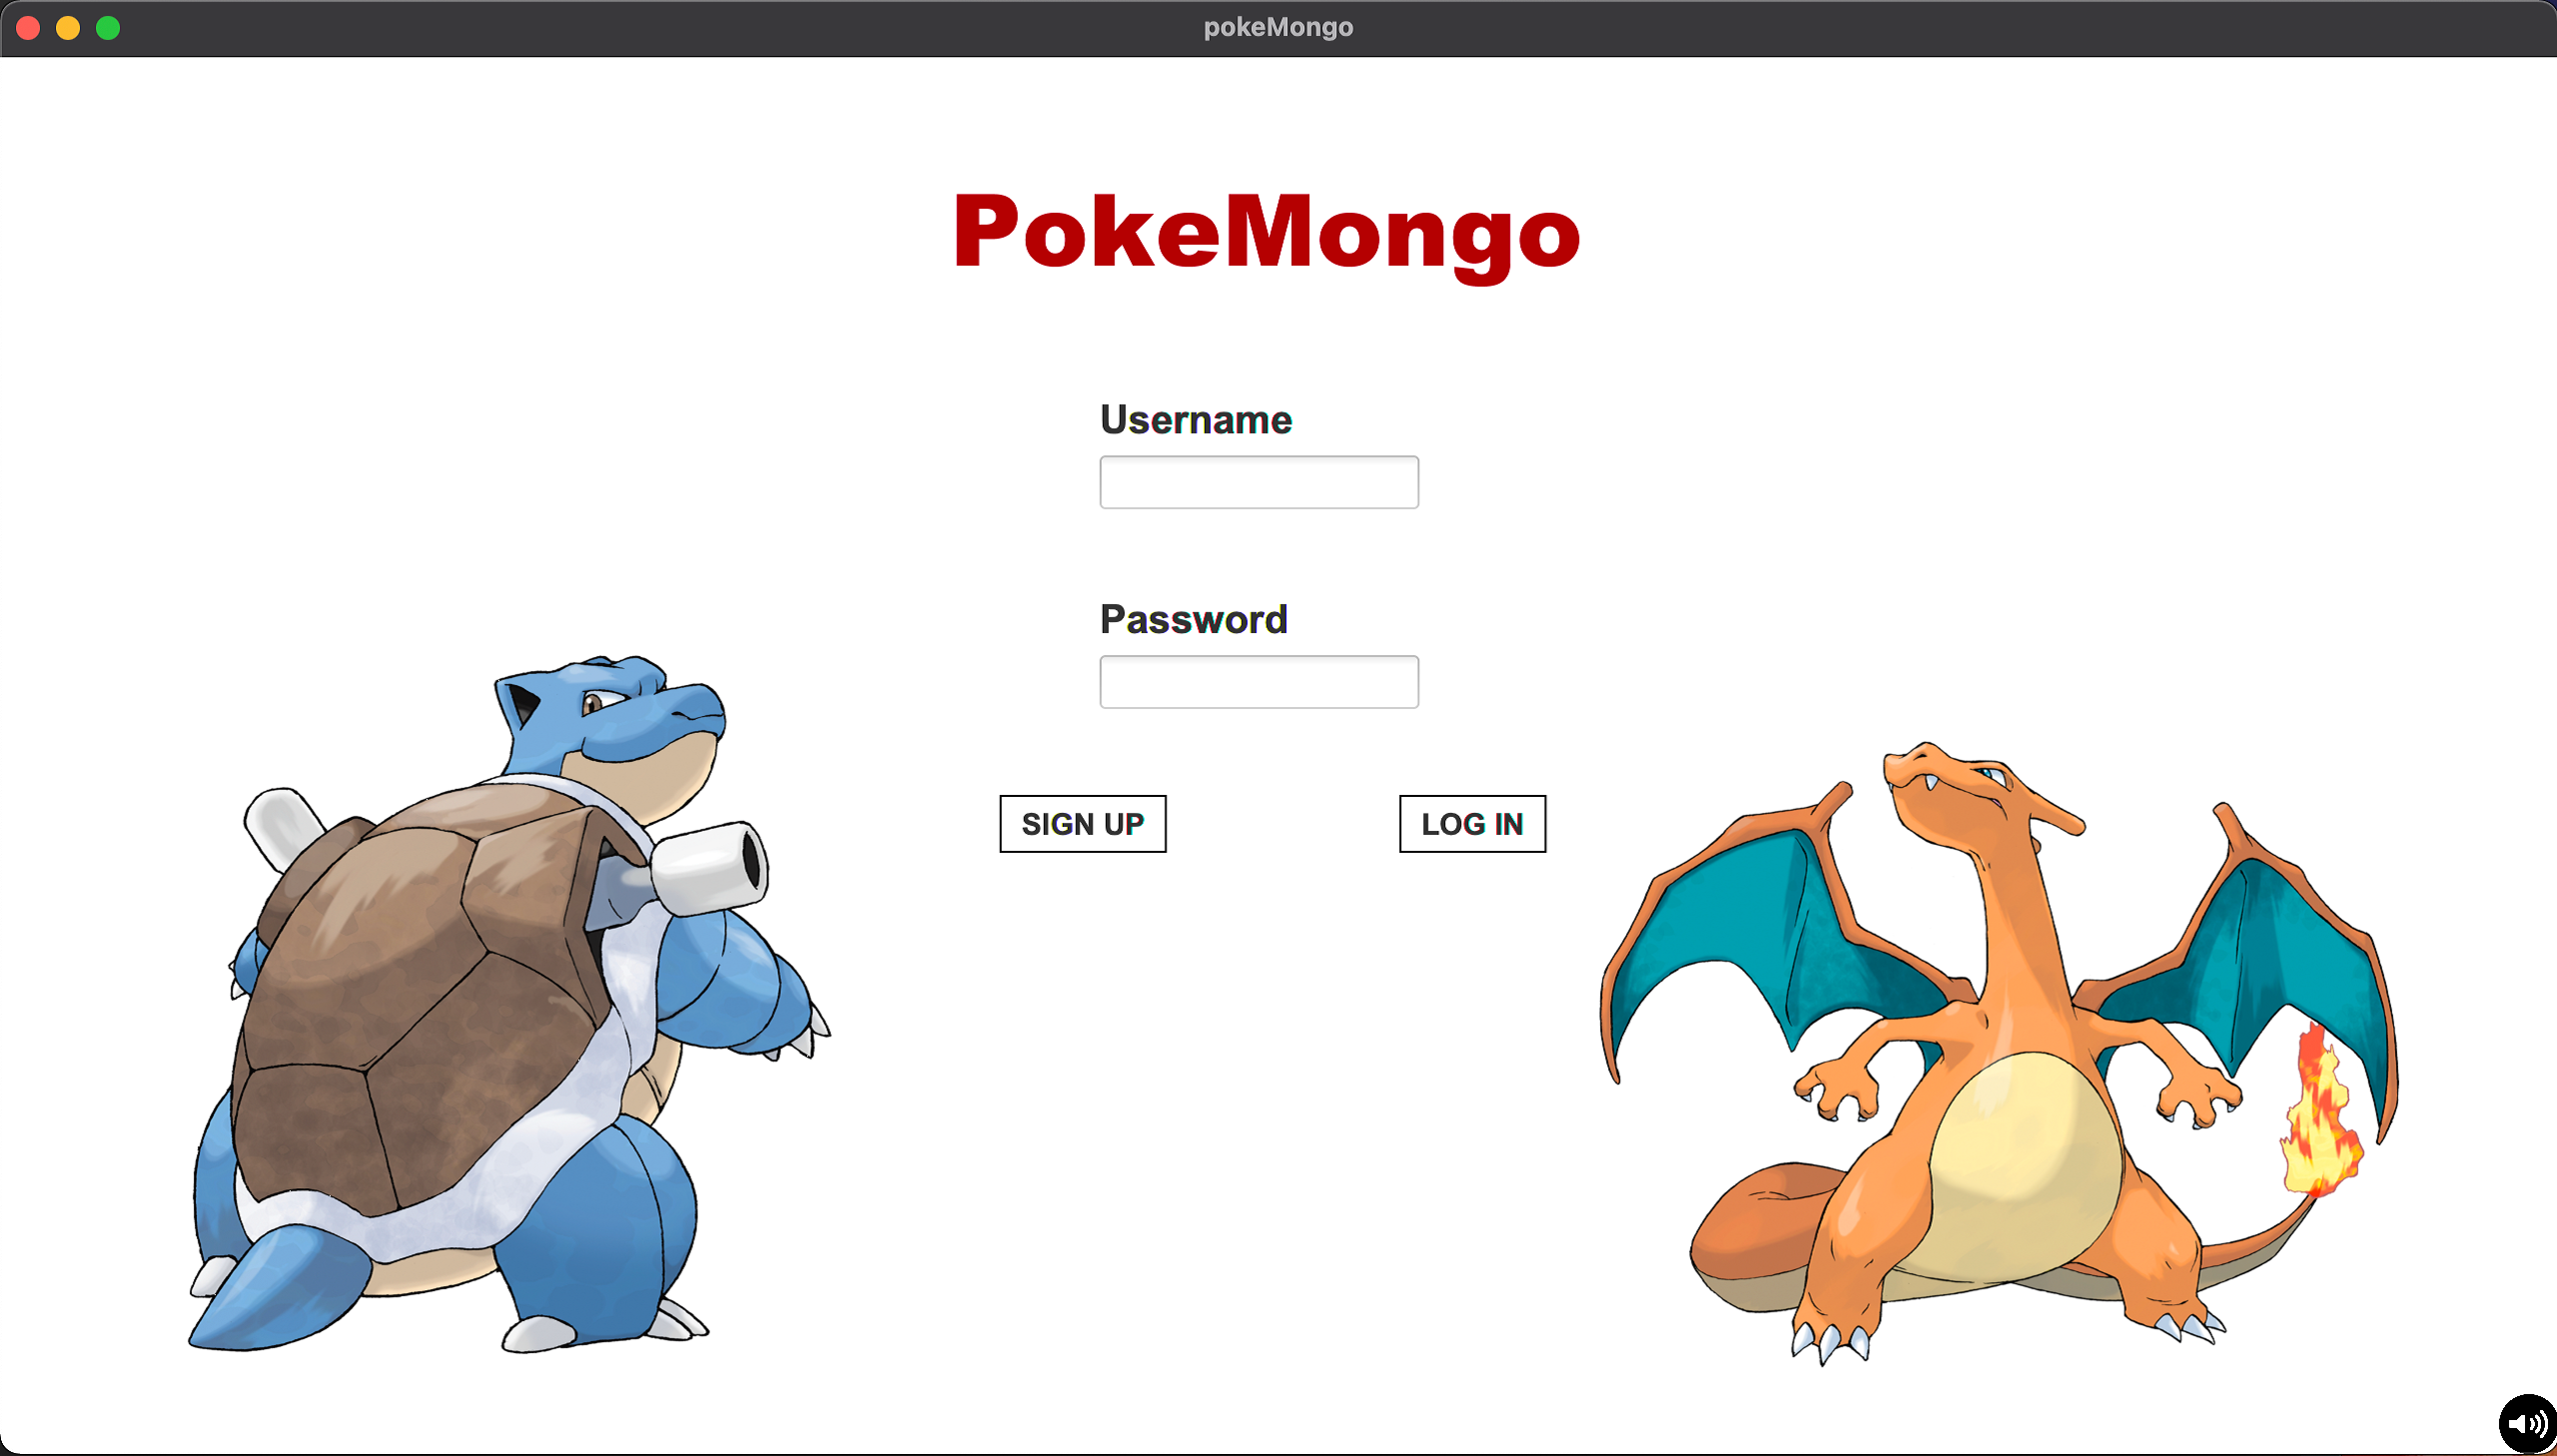
\includegraphics[width= \textwidth]{img/userManual/login.png}
	\caption{Login Page}
\end{figure}
User can fill the textfields and press the LOG IN button in order to log in to the application or they can sign up to the service by pressing the SIGN UP button, compiling the registration form and then pressing the SUBMIT BUTTON. If there are no errors red popups won't be shown and the User can turn back to the Login page by pressing the BACK button.
\begin{figure}[H]
	\centering
	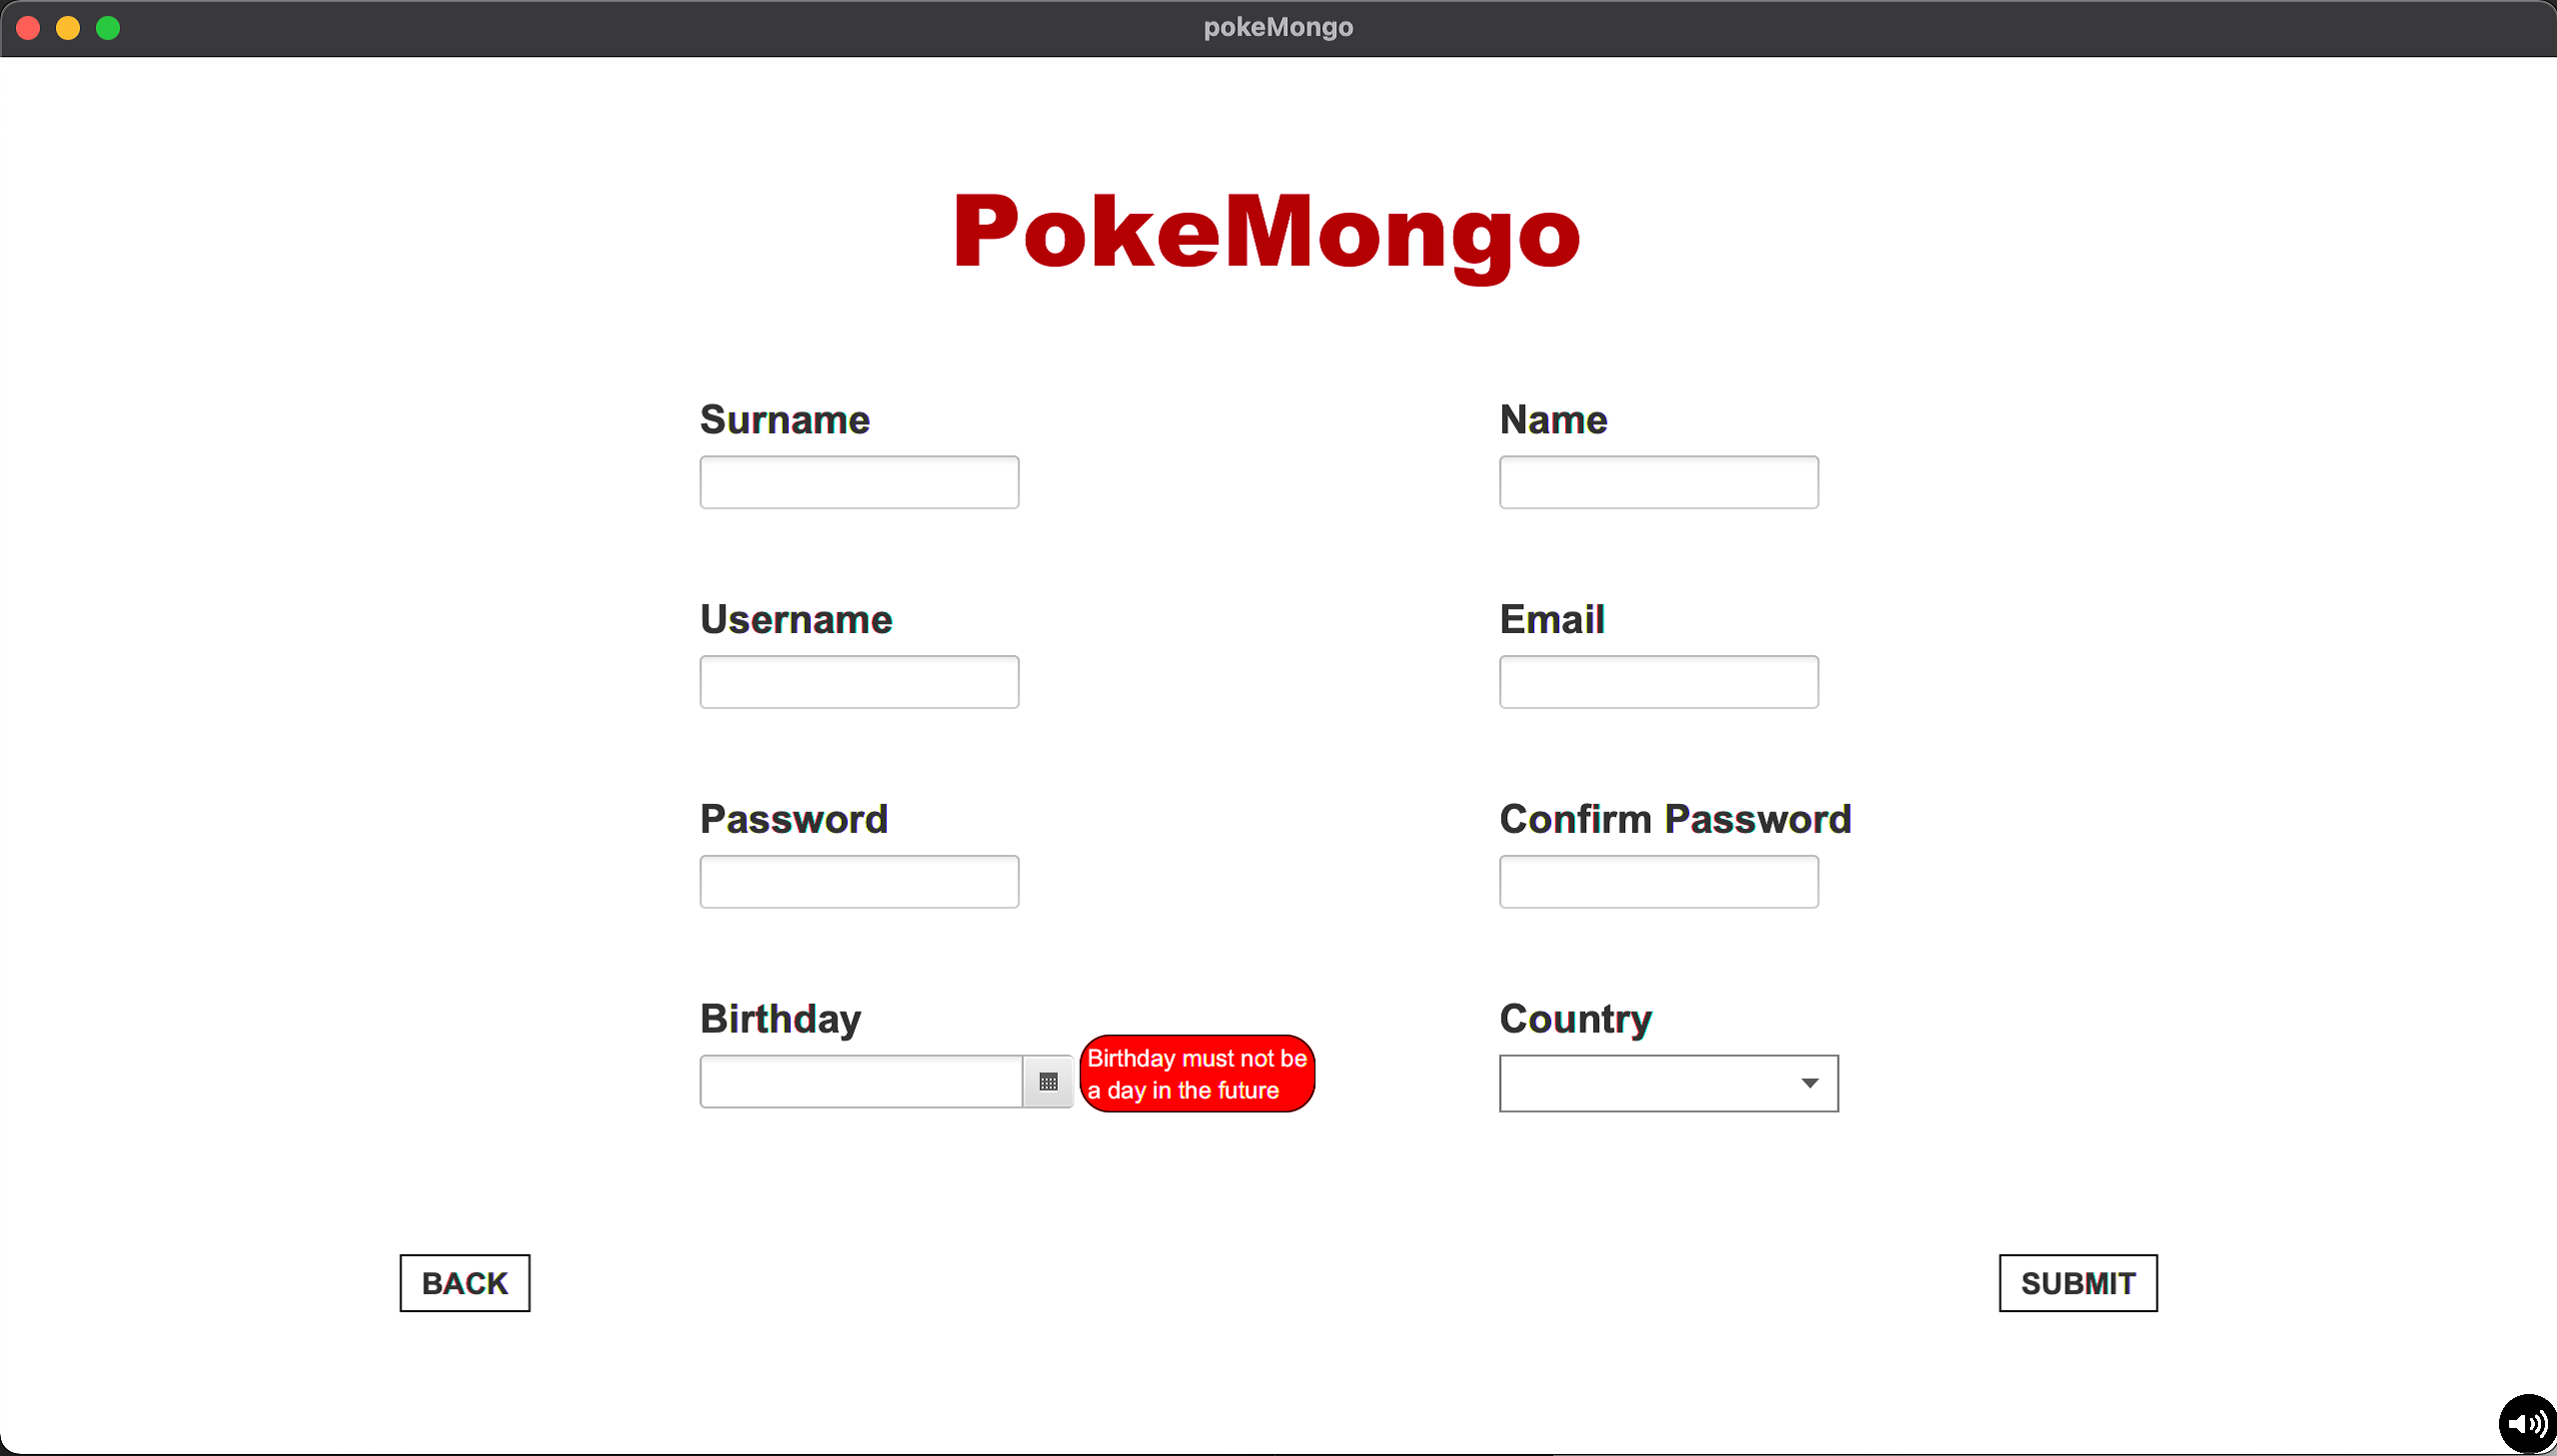
\includegraphics[width=\textwidth]{img/userManual/registration.png}
	\caption{Registration Page}
\end{figure}
The registration could only be made by \textit{Normal Users}, the \textit{Admins} credentials will be given to the client company.
After the login the following Page will be shown.
\begin{figure}[H]
	\centering
	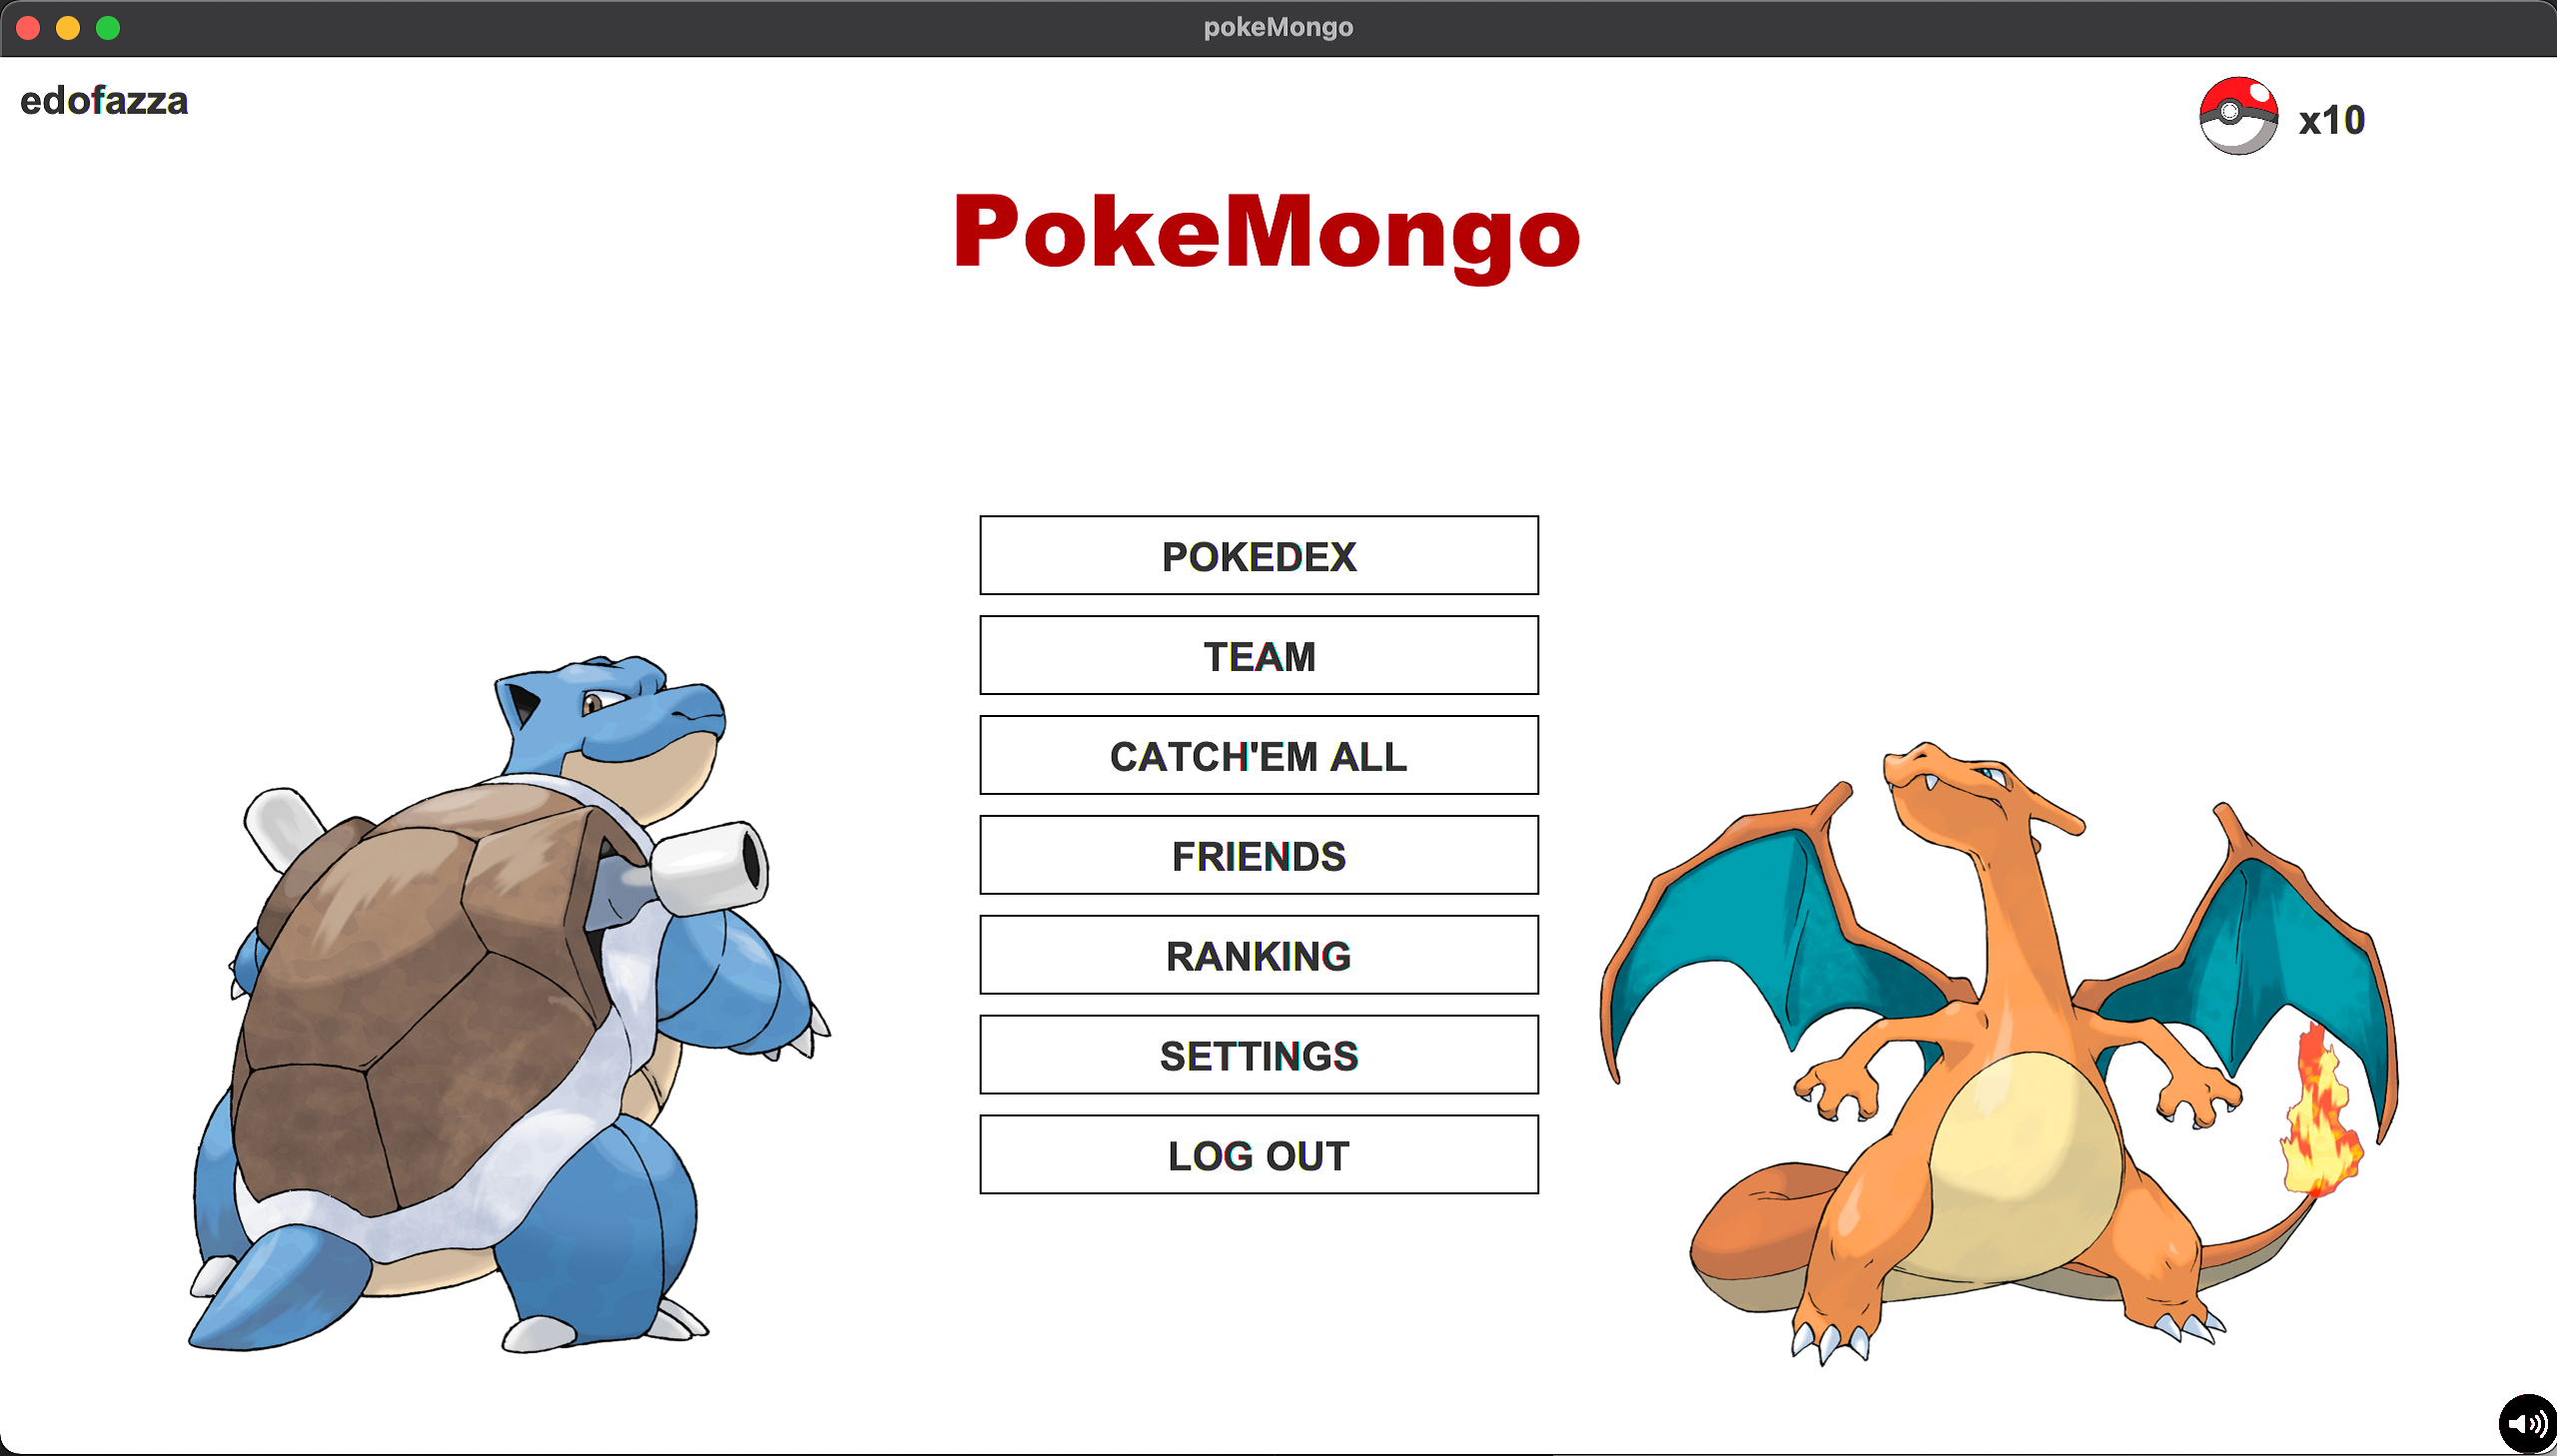
\includegraphics[width=\textwidth]{img/userManual/main.png}
	\caption{HomePage}
\end{figure}
Notice that in the top-left corner is visible the \textit{username} whereas in the top-right corner the number of \textit{dailypokeball}. These items will be always visible when a user is logged to the application. On the bottom-right corner there is a button which, if pressed, stops the music played at the launch of the application.
\subsubsection{Pokedex}
The Pokedex will help the \textbf{User} to discover new Pokemons and to know more about them.
\begin{figure}[H]
	\centering
	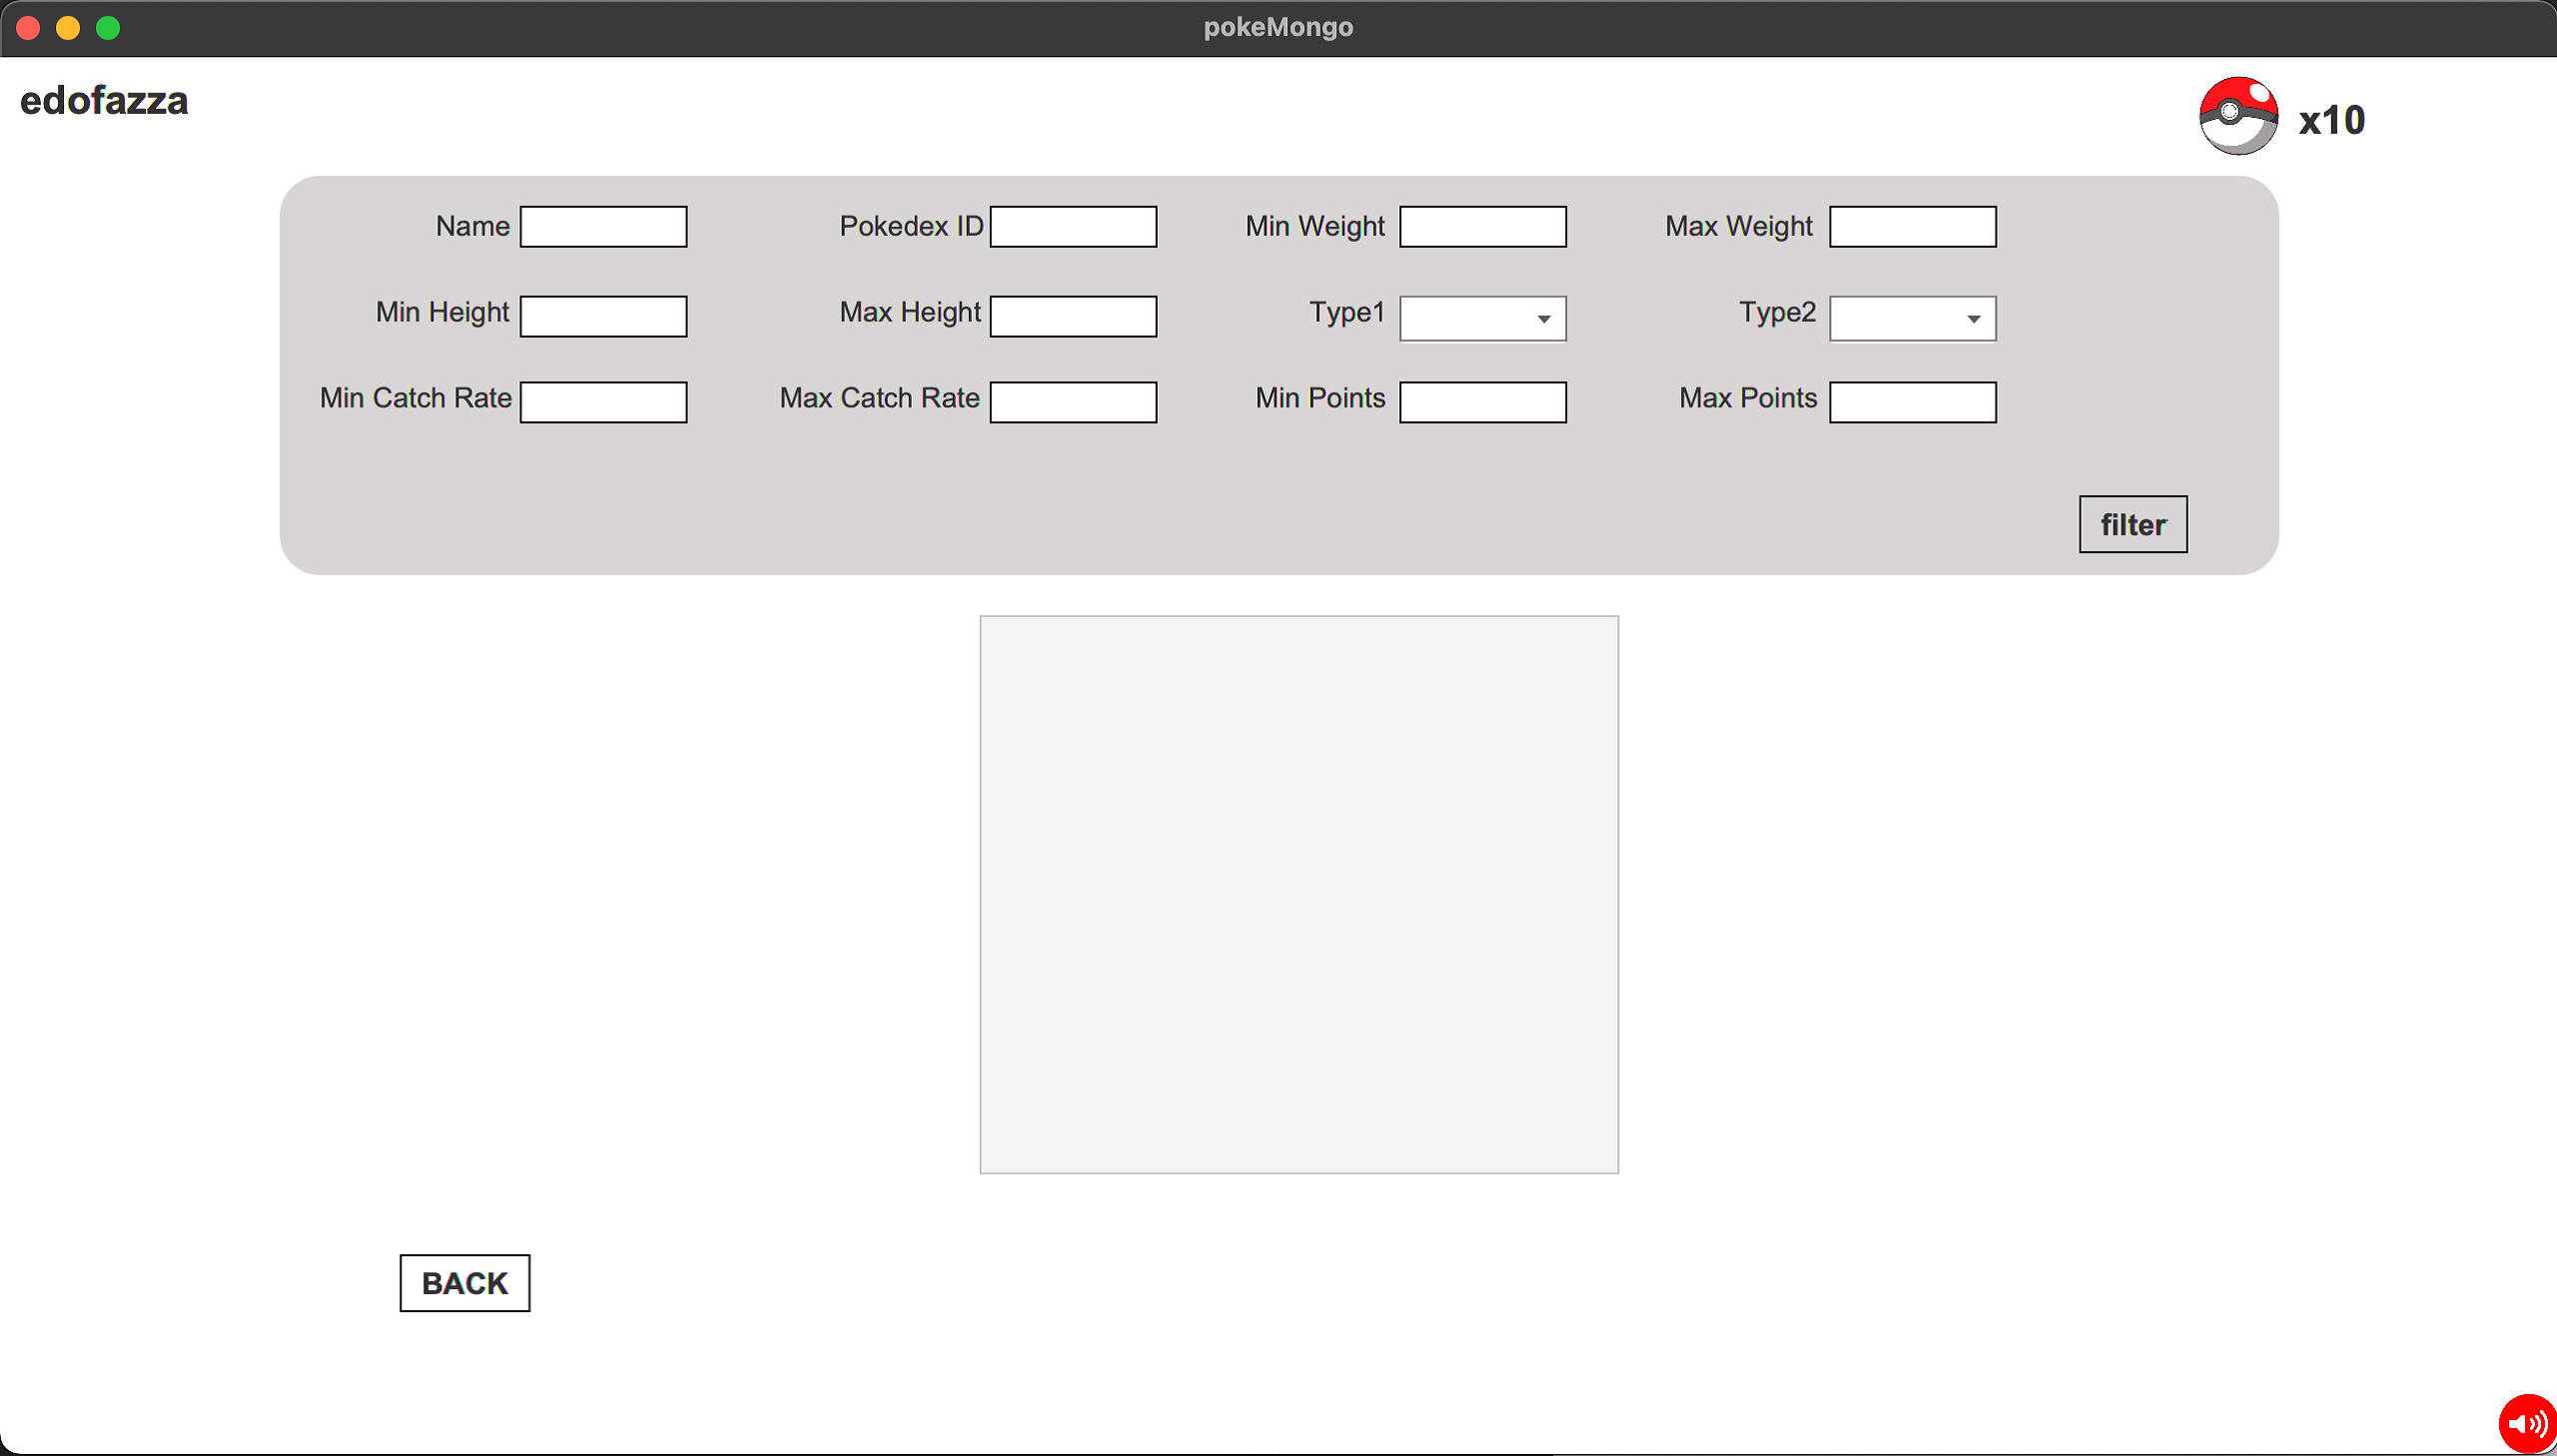
\includegraphics[width=\textwidth]{img/userManual/pokedex.png}
	\caption{Pokedex Page}
\end{figure}

The User can use as many parameters as he want for searching, but at least one should be used. After setting some filters the User must click the FILTER button in order to get the search results. In the following image there is an example of the usage of the Pokedex.
\begin{figure}[H]
	\centering
	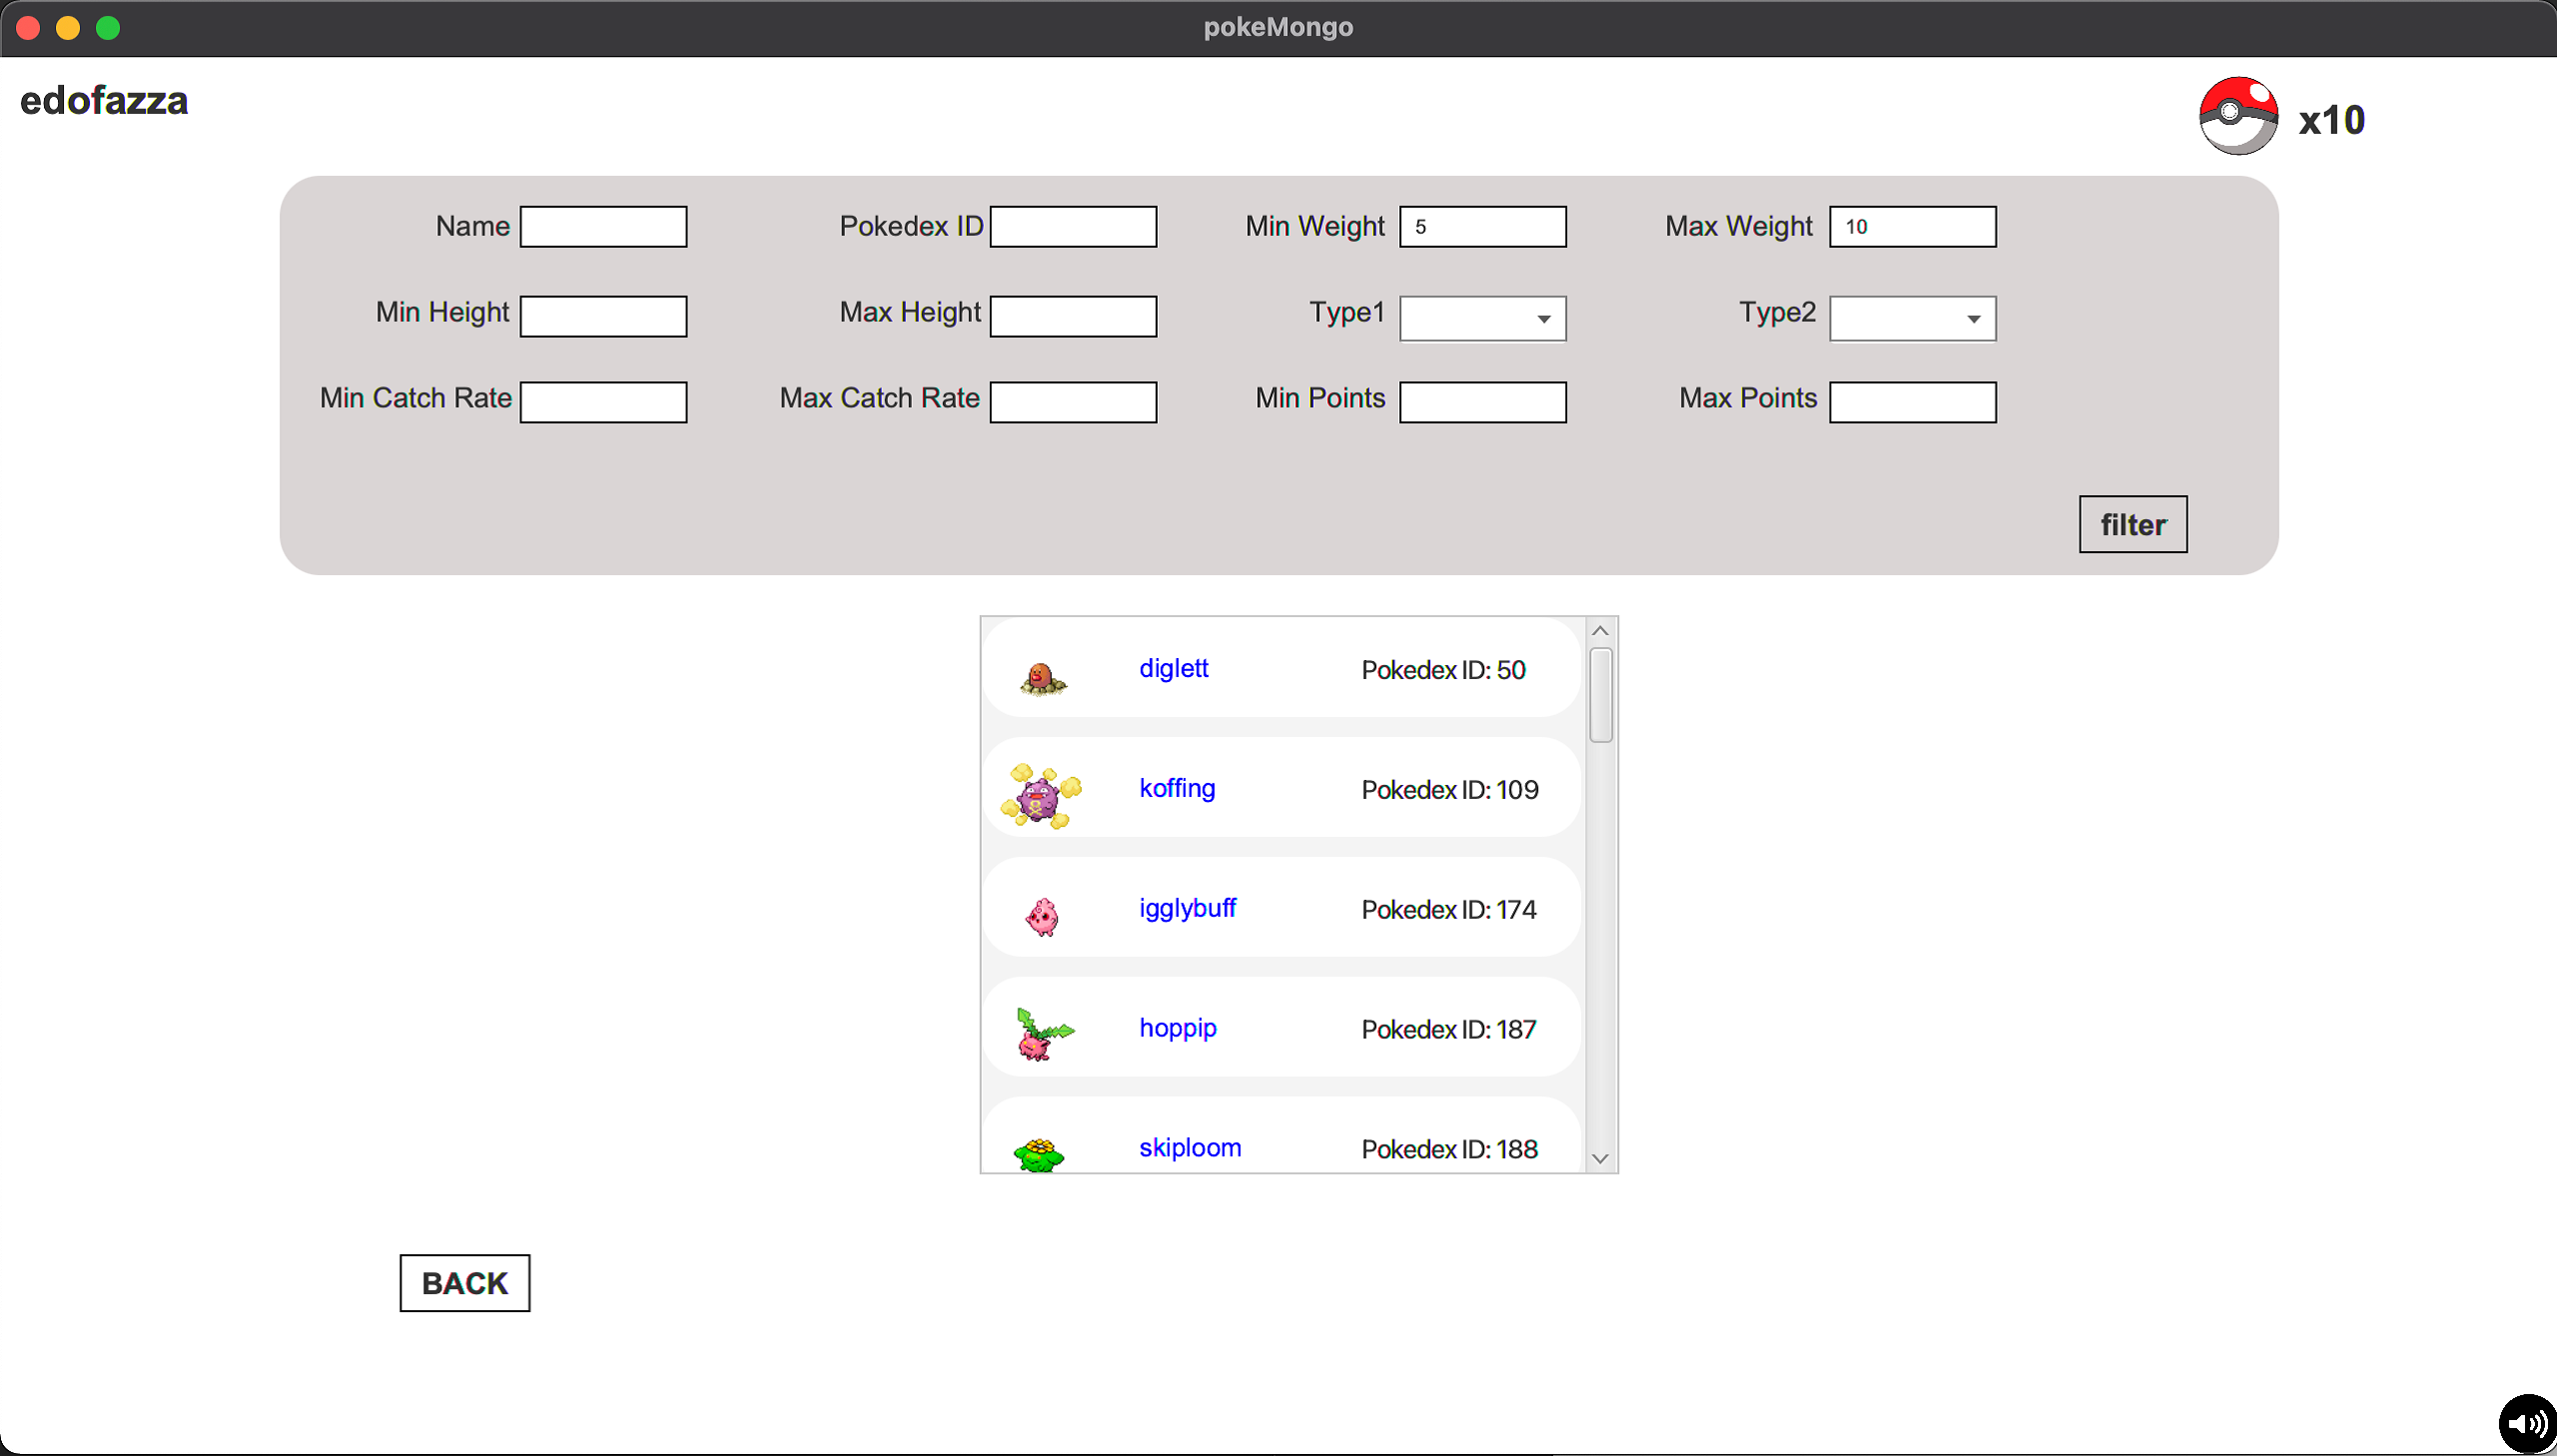
\includegraphics[width=\textwidth]{img/userManual/pokedex2.png}
	\caption{Pokedex Page after filtering}
\end{figure}
\textbf{Notice that if there is no internet connection no image will be loaded but the application will still work}. The BACK button will redirect again to the homepage. If the \textbf{User} \textbf{clicks} on the name of the \textbf{Pokemon}, a popup will be shown. 
\begin{figure}[H]
	\centering
	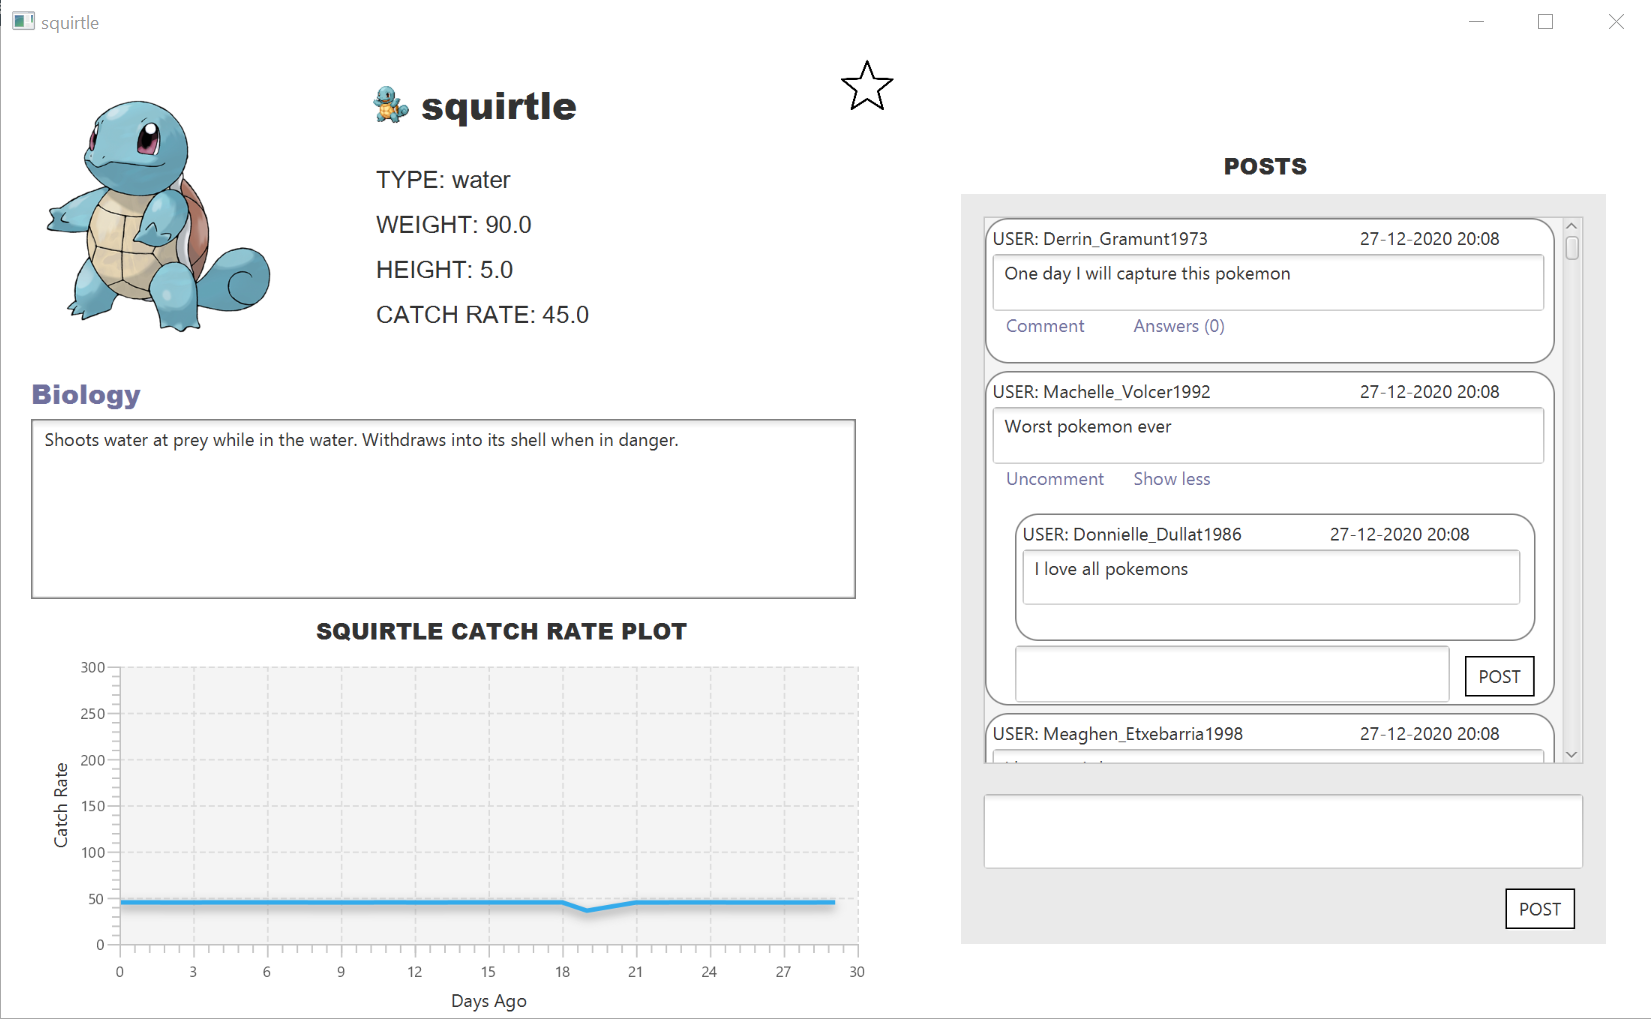
\includegraphics[width=\textwidth]{img/userManual/pokemon_info.png}
	\caption{Pokemon Info's Window}
\end{figure}
In the popup all the information regarding a single \textbf{Pokemon} are shown. At the left bottom you can see a plot in which it’s displayed the evolution of the catch rate of selected \textbf{Pokemon} in the last thirty days. The STAR is a special button, if you click on it you will make that \textbf{Pokemon} one of your favorites. The star will turn yellow. To remove it from favorites you have just
to click on it, the star will turn than white again. On the right there is the \textit{Post Section} where the user Can write some posts about the pokemon or reply to other posts. If the user is the owner of a post/comment he can delete it, by clicking to the red writing DELETE inside the post or the reply.
\subsubsection{Team}
The \textit{team page} lets the \textbf{User} handle his personal team.
There will be shown the \textbf{captured Pokemons}. 
\begin{figure}[H]
	\centering
	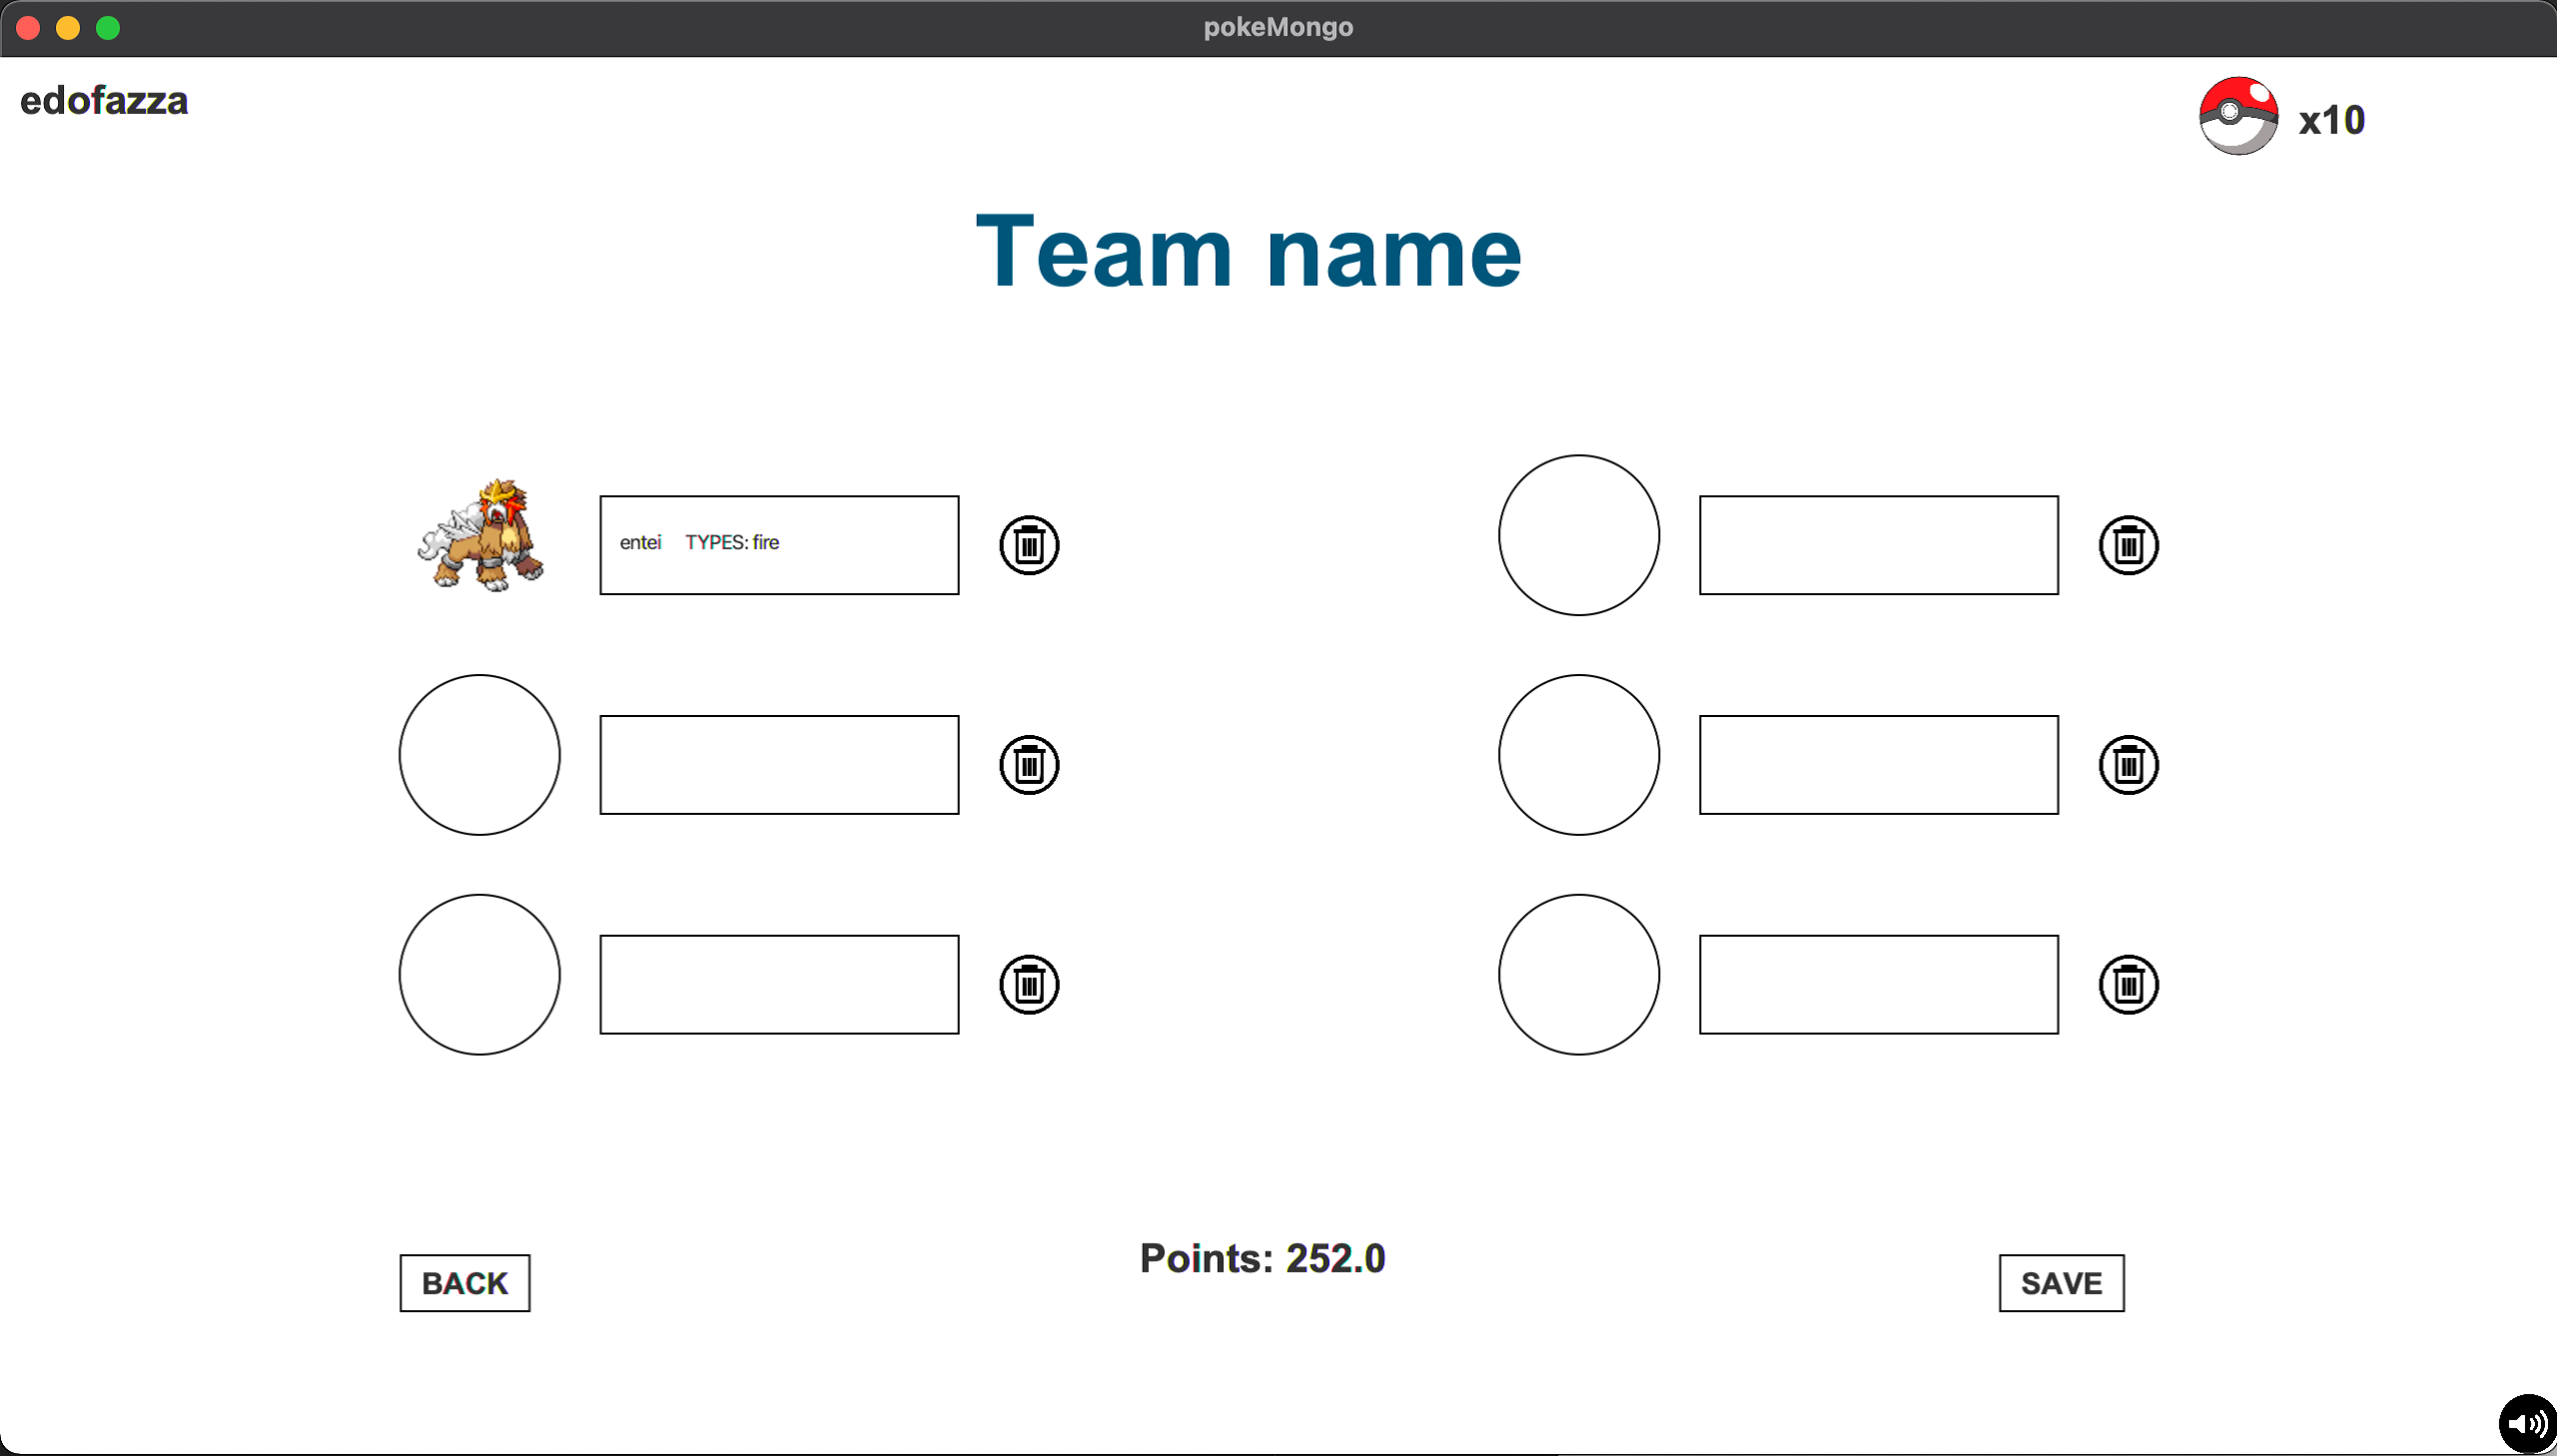
\includegraphics[width=\textwidth]{img/userManual/team.png}
	\caption{Team Page}
\end{figure}
The TRASH button near the slot can eliminate the Pokemon from the team (don’t worry! You won’t kill it, you’ll just free it). The team name is displayed at the top and is editable. At the bottom are shown the team points. Any changes in the team should be saved to completely store them in a persistent way, to do the \textbf{User} must press the SAVE button.
\subsubsection{Catch'em All}
In this page the \textbf{User} can capture other \textbf{Pokemon}. In order to do so the User must type the \textbf{Pokemon} name or click on the favourite table in order to copy quickly the name of a favourite one. Then he must choose a slot to capture the \textbf{Pokemon}, where this slot must be free, and, at the end, he must click on the TRY TO CATCH button in order to make the capture attempt, which success depends on the odd of the pokemon. The result of the attempt will be shown below. The \textbf{User} has a limited number of \textit{pokeballs} (for instance, 10 pokeballs per day), which represent the number of attemps to capture a Pokemon. If no pokeball are left the User can't perform the capture.
\begin{figure}[H]
	\centering
	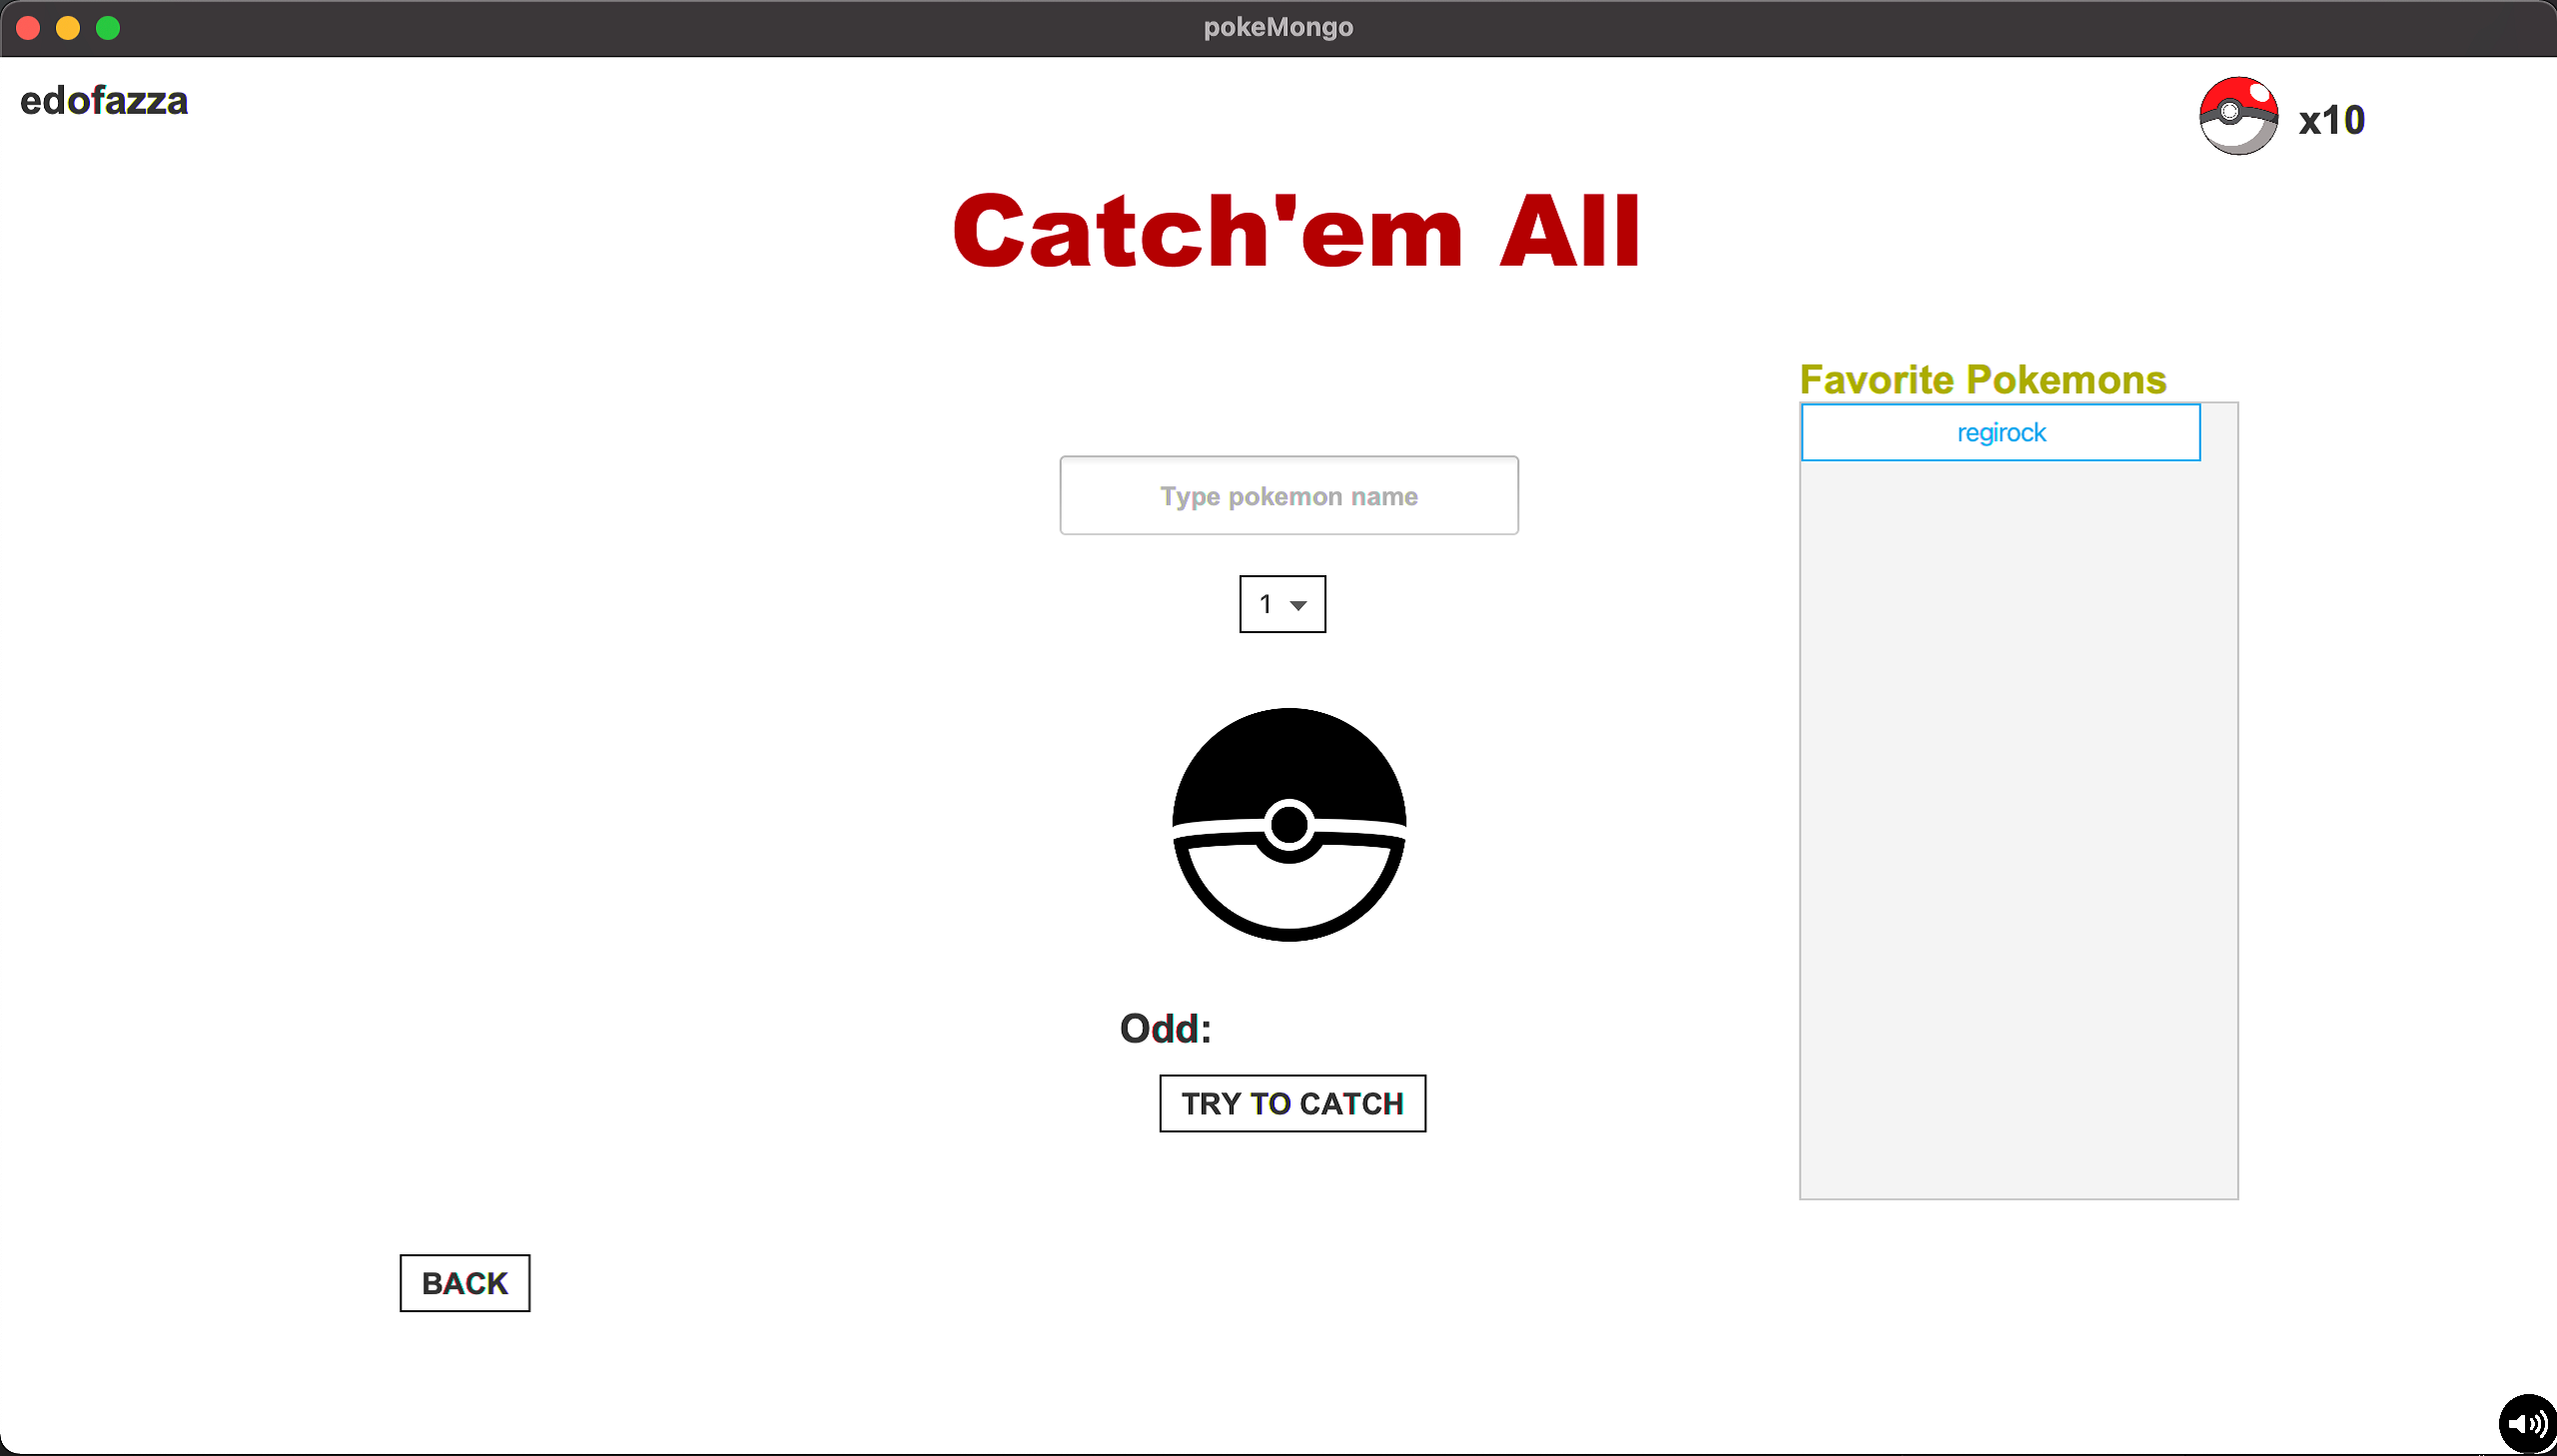
\includegraphics[width=\textwidth]{img/userManual/catch.png}
	\caption{Cathc'em All Page}
\end{figure}
\subsubsection{Friends}
In this page are shown information about the friends, people who the User follows, of a \textbf{User}. 
\begin{figure}[H]
	\centering
	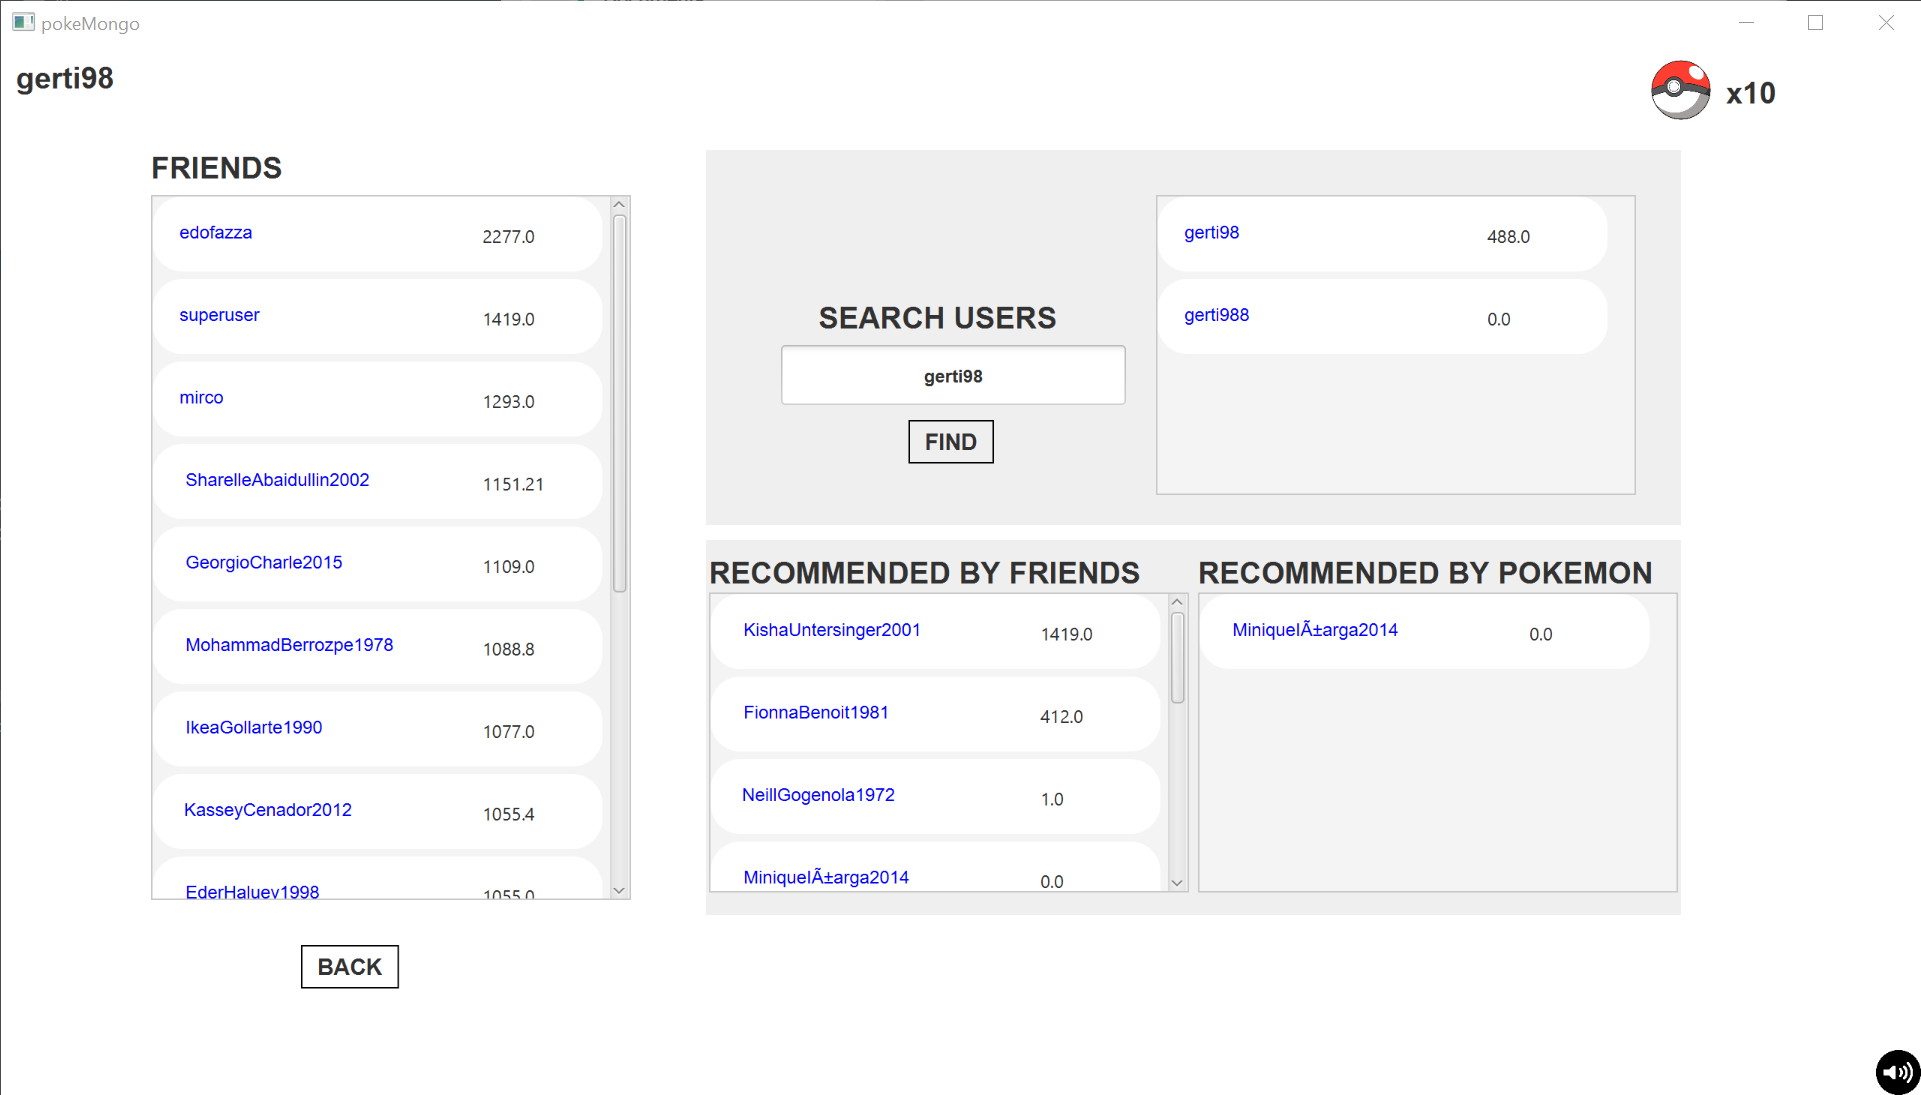
\includegraphics[width=\textwidth]{img/userManual/friends.png}
	\caption{Friends Page}
\end{figure}
In the left Pane is shown the friends list, in the top-right pane is possible to search a particular user by username, while in the bottom-left panes are shown some suggested Users to follow based on the people followed or the pokemon liked.
By clicking on a User name will be shown another Popup as the following:
\begin{figure}[H]
	\centering
	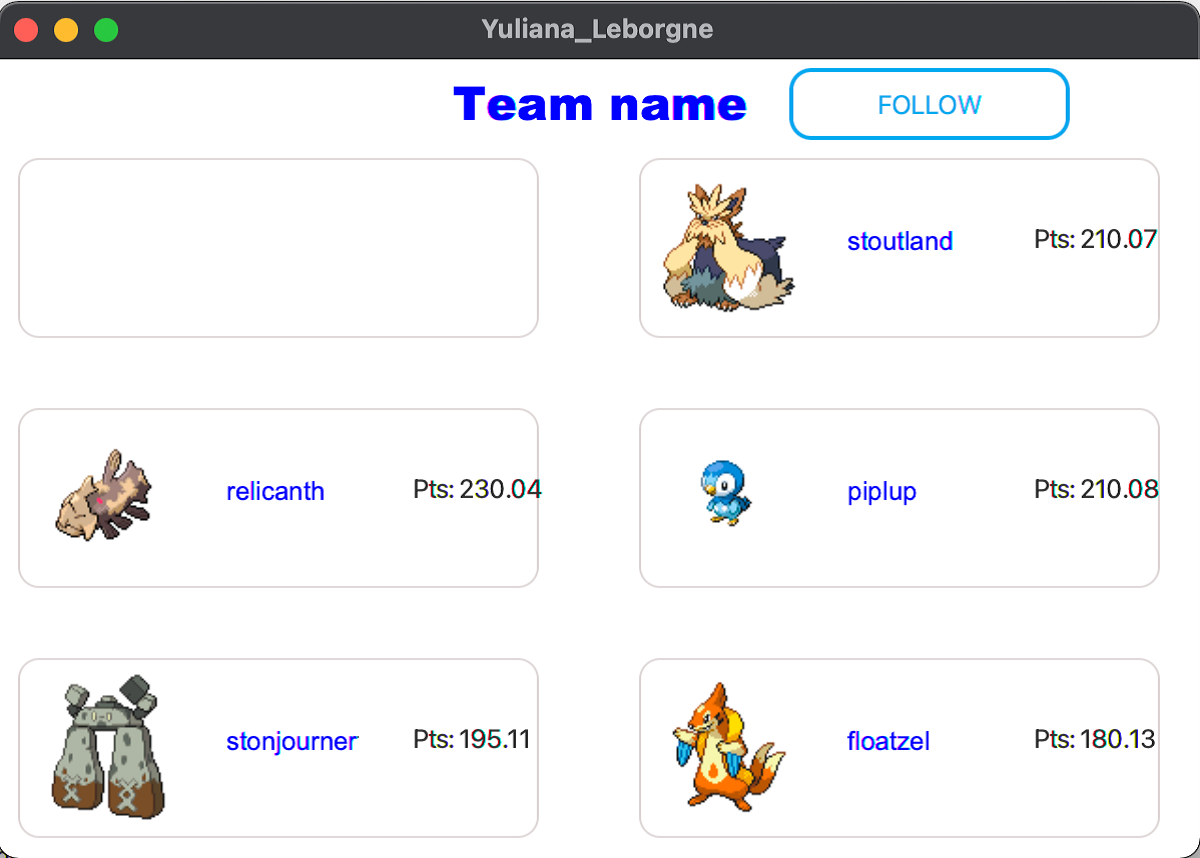
\includegraphics[width=\textwidth]{img/userManual/team_popup.png}
	\caption{User Team Popup}
\end{figure}
In which the team composition and the team name of a particular \textbf{User} is shown. By pressing the FOLLOW button at the top right corner that particular \textbf{User} is added to the friends list and the button will turn into an UNFOLLOW button, which will permit to delete a User from the friends list.
\subsubsection{Ranking}
In this page are displayed different types of ranking: the Most Used Pokemon and the Best Teams, which can be filtered by Country, and the Best Teams among friends. In the following image is shown how this page is displayed in the application.
\begin{figure}[H]
	\centering
	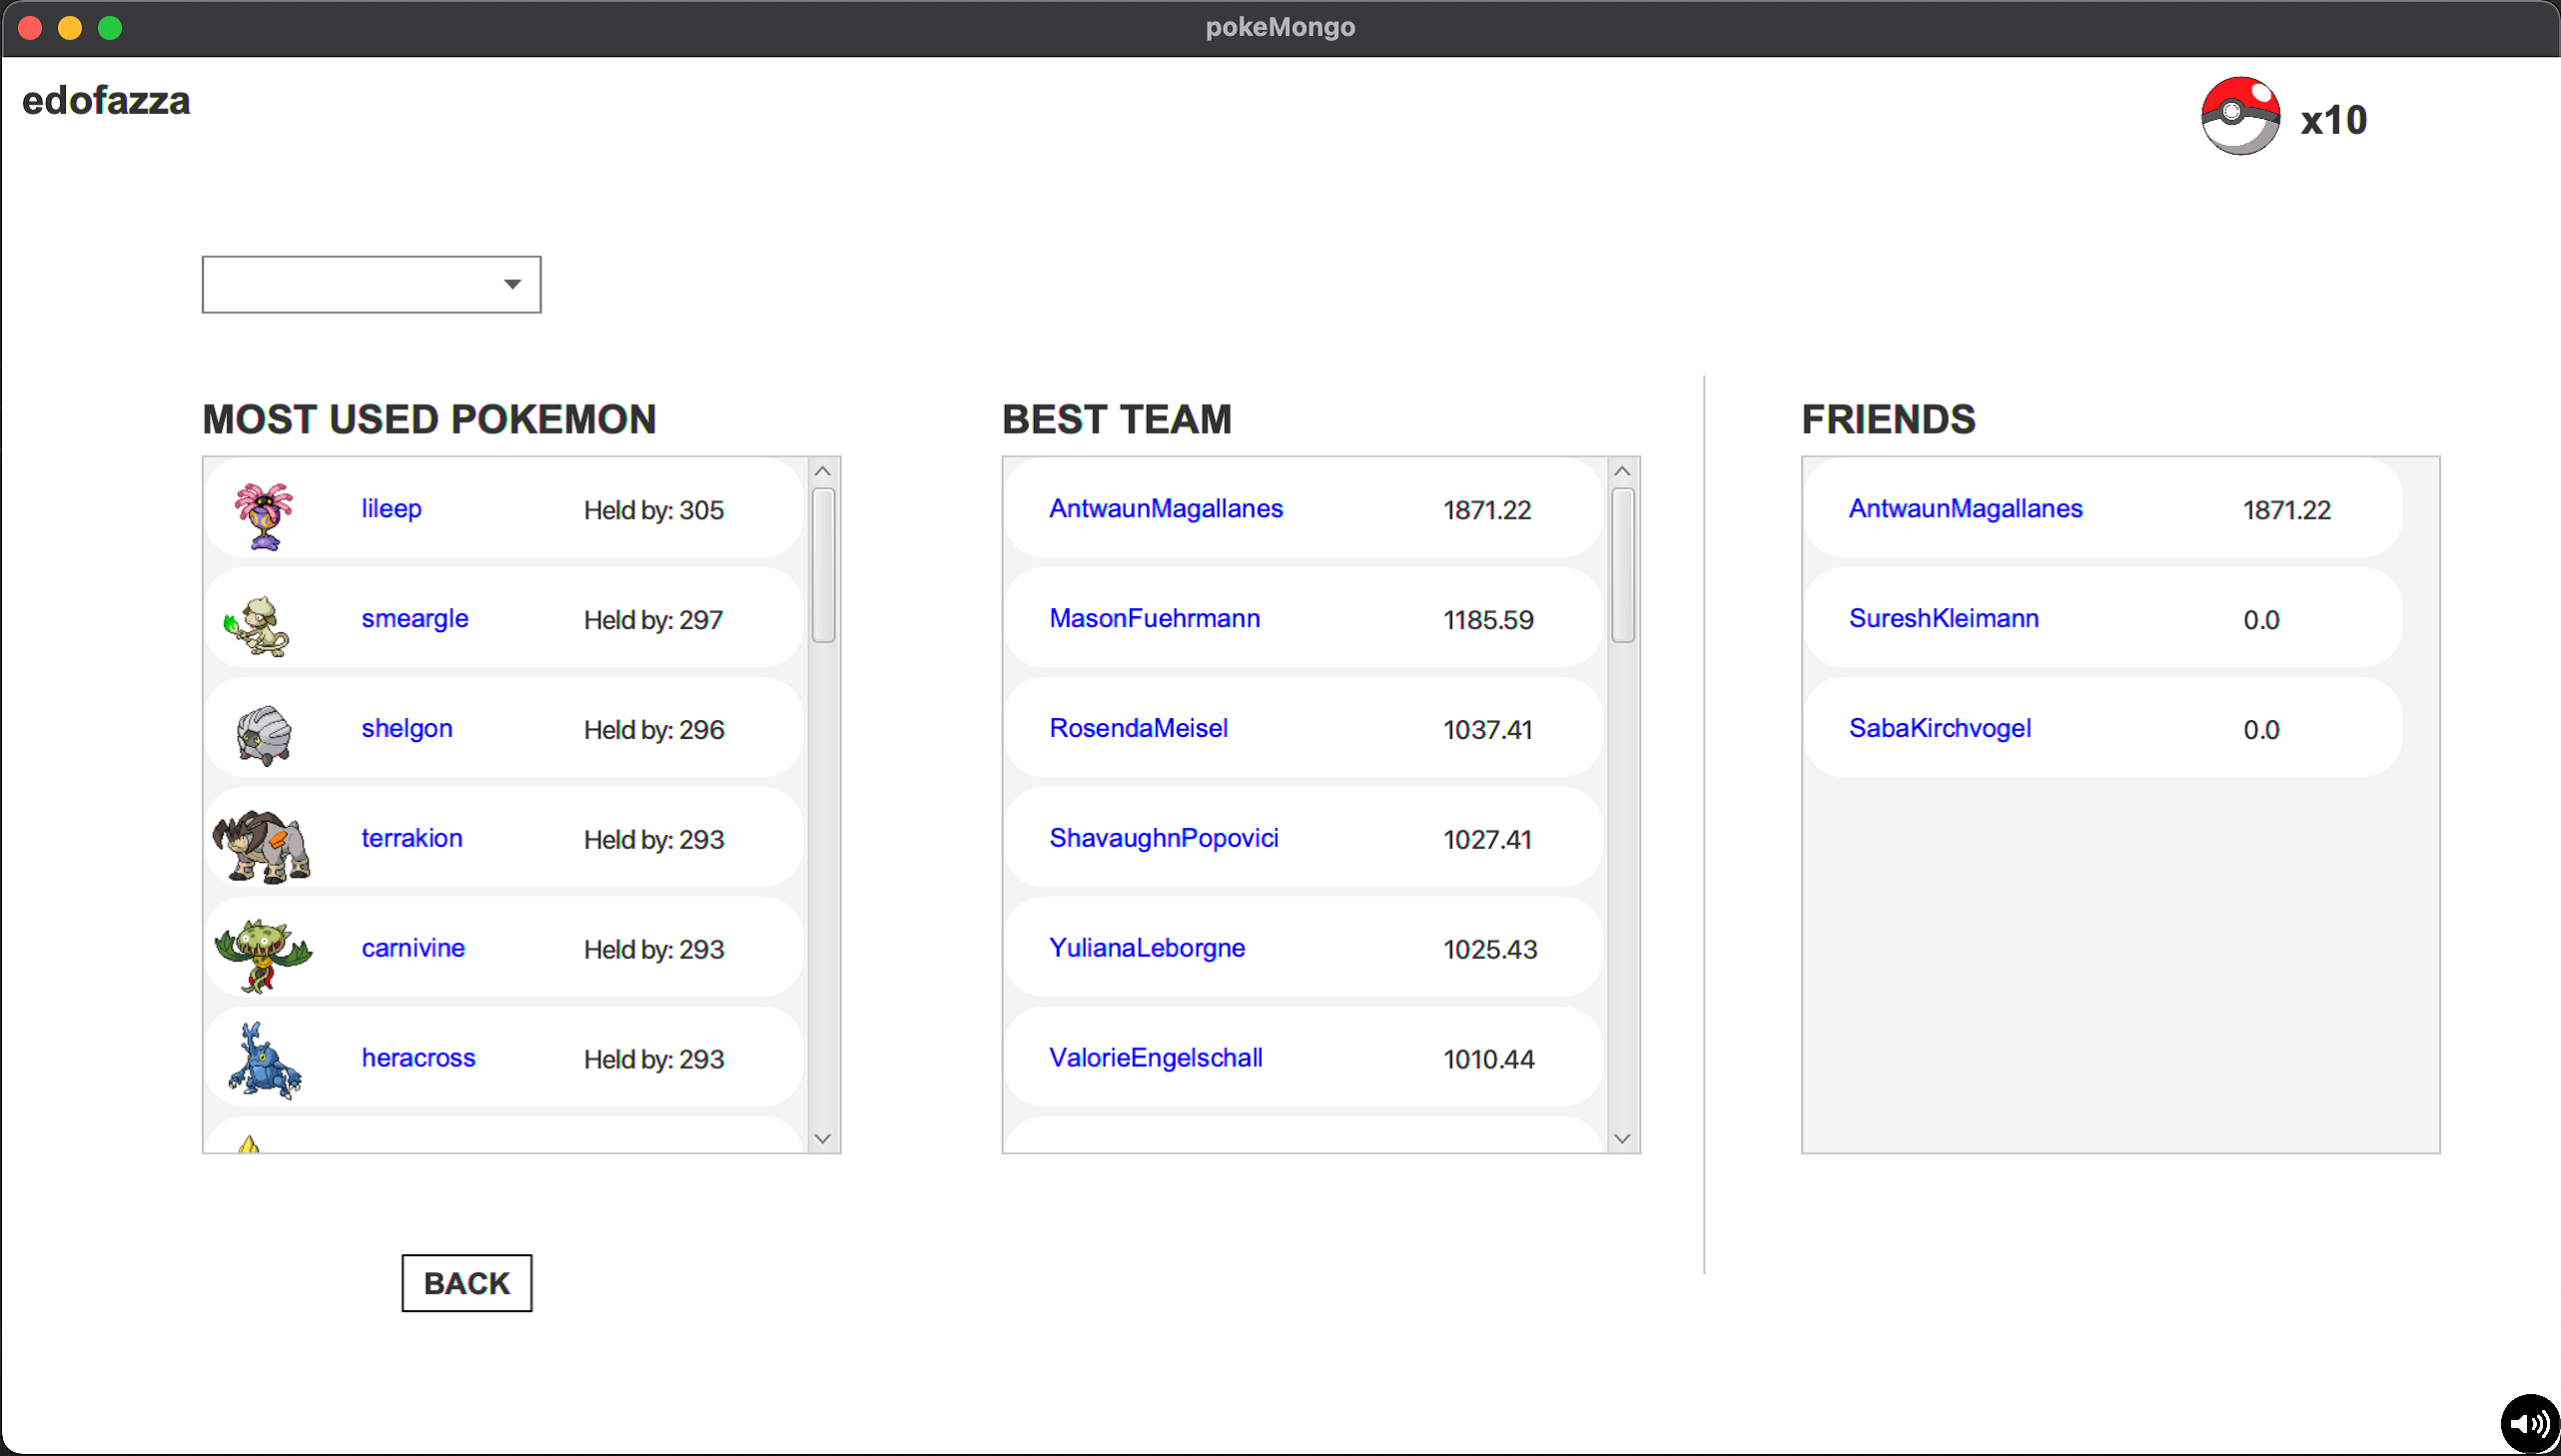
\includegraphics[width=\textwidth]{img/userManual/ranking.png}
	\caption{Ranking Popup}
\end{figure}
By clicking on the top-left combobox is possible to perform the Country filtering of the Rankings (the friens one won't be affected).

\subsubsection{Settings}
In this page is possible to modify some User registration information like the email, the password and the country.
\begin{figure}[H]
	\centering
	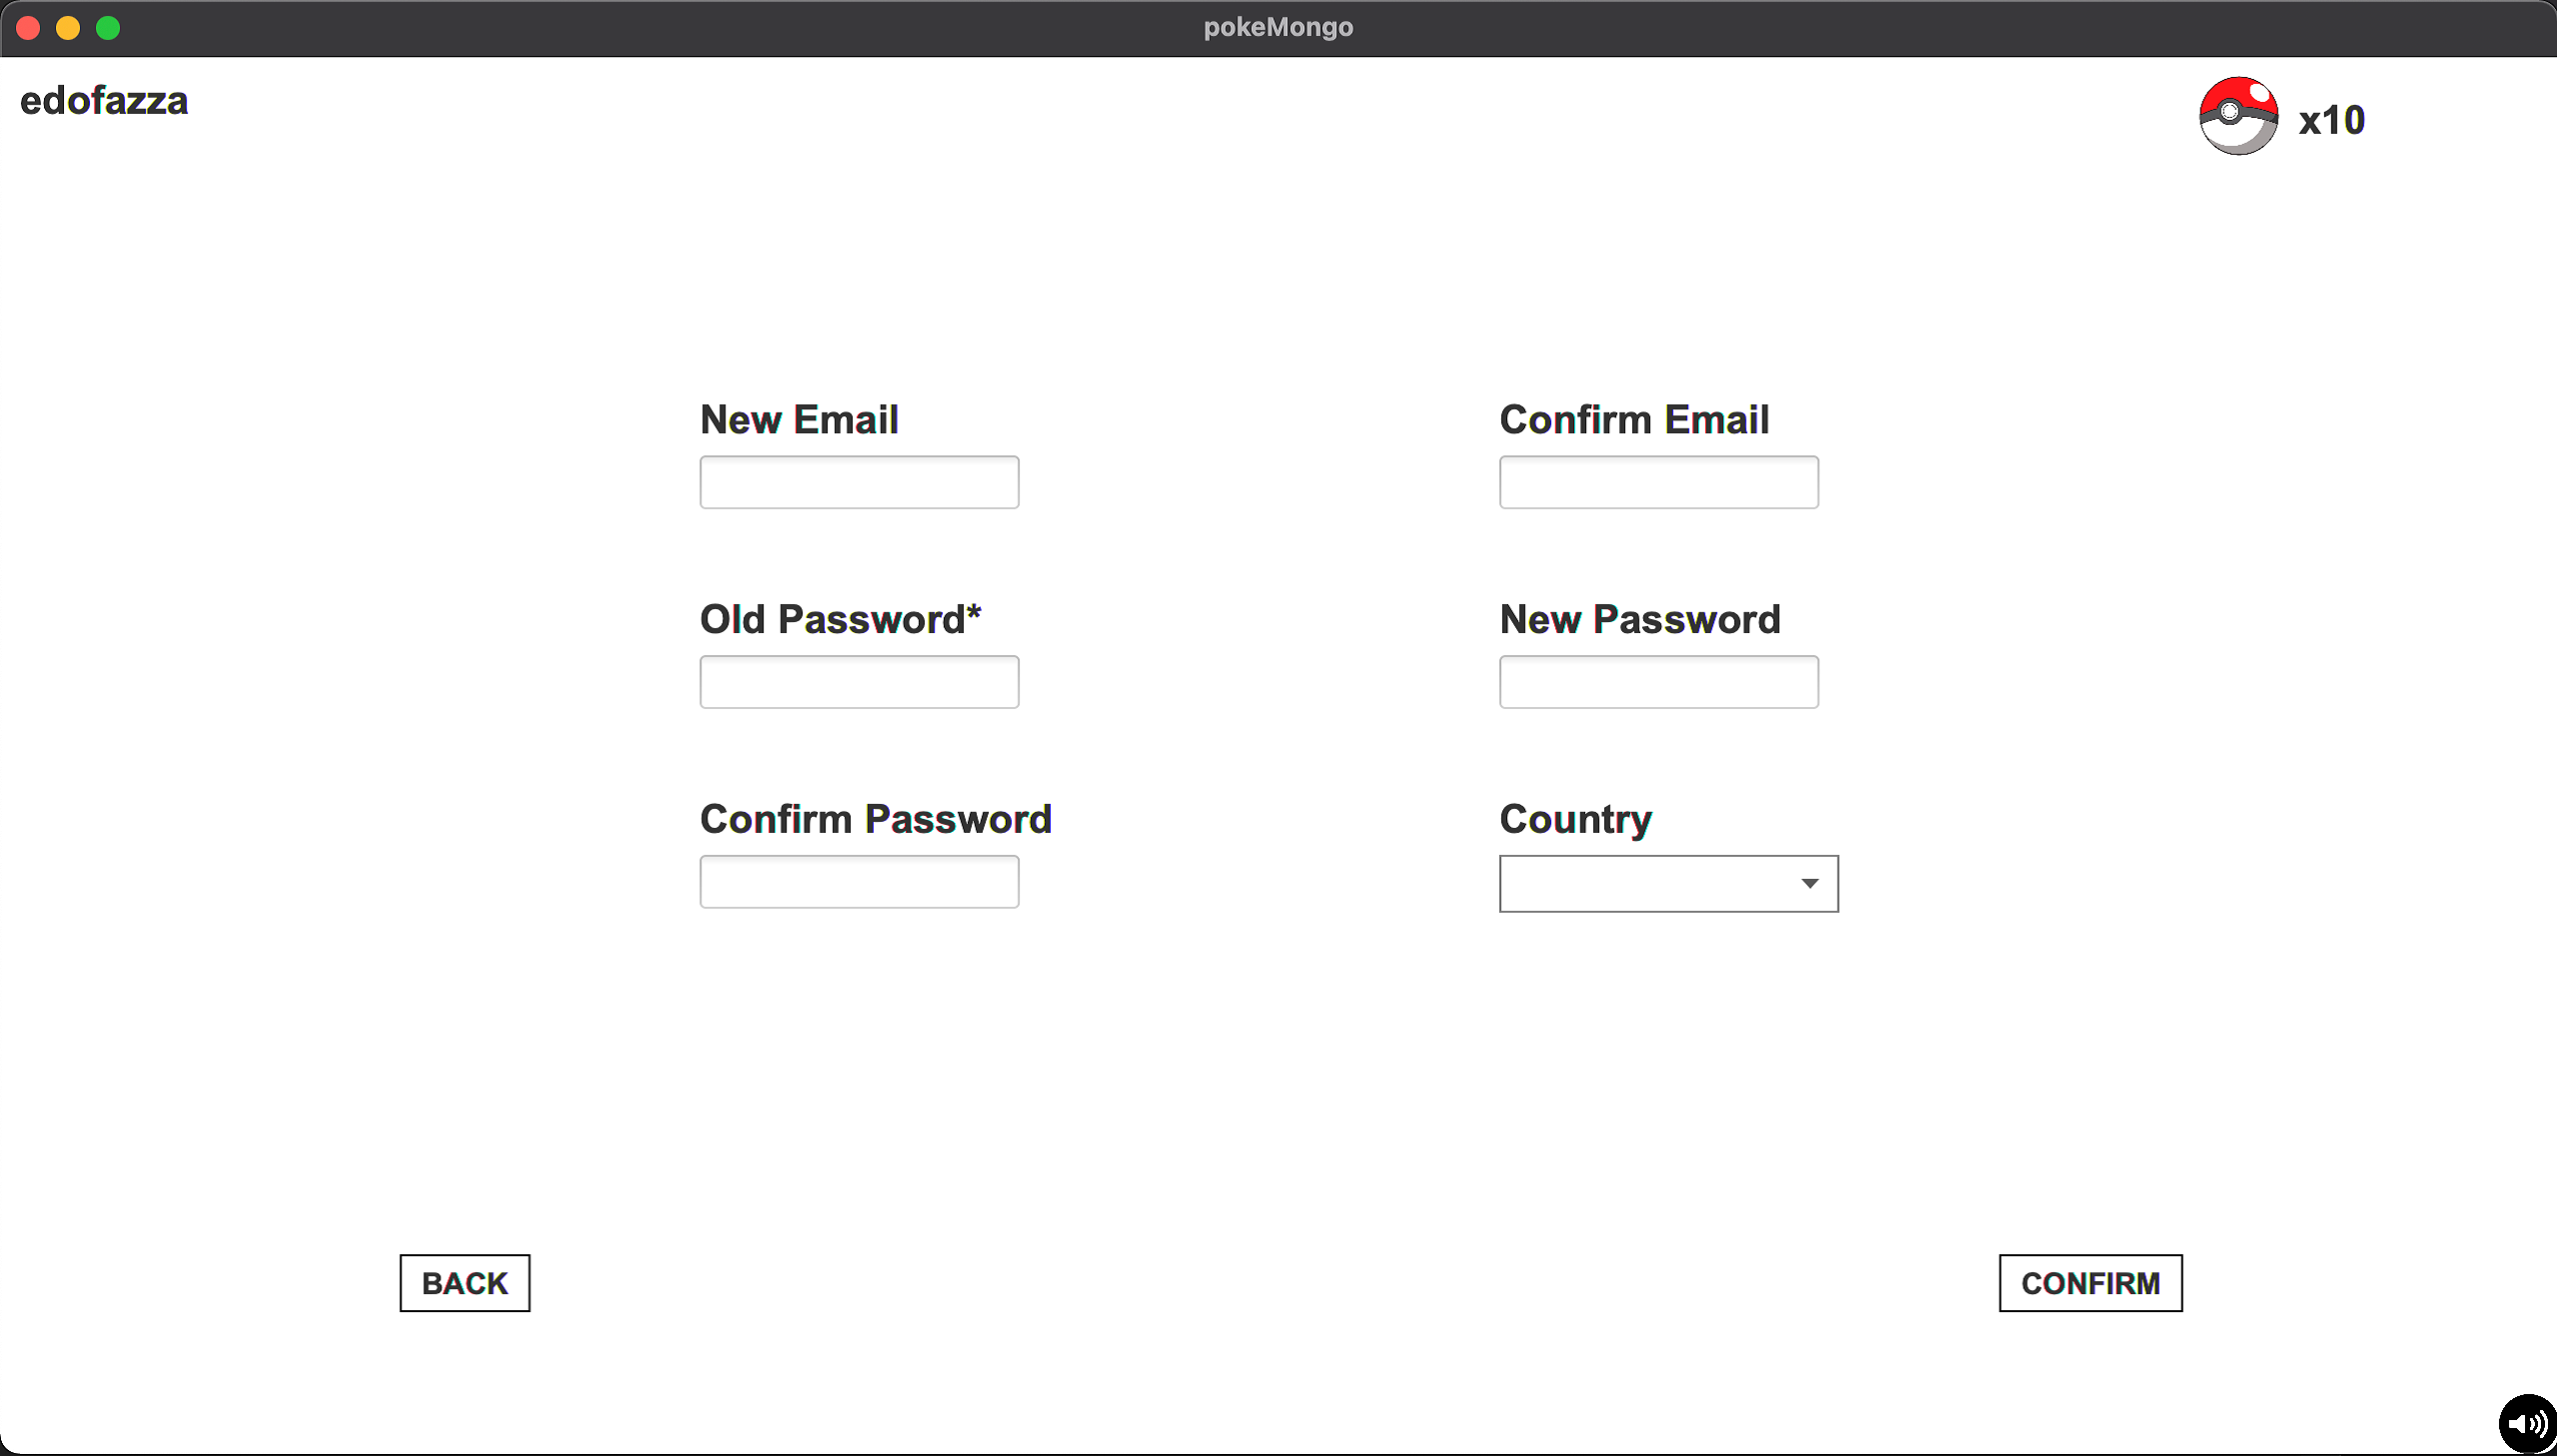
\includegraphics[width=\textwidth]{img/userManual/settings.png}
	\caption{Settings Page}
\end{figure}
\subsection{Admin Manual}
\subsubsection{Admin Homepage}
After the login of the admin the following homepage will be shown.
\begin{figure}[H]
	\centering
	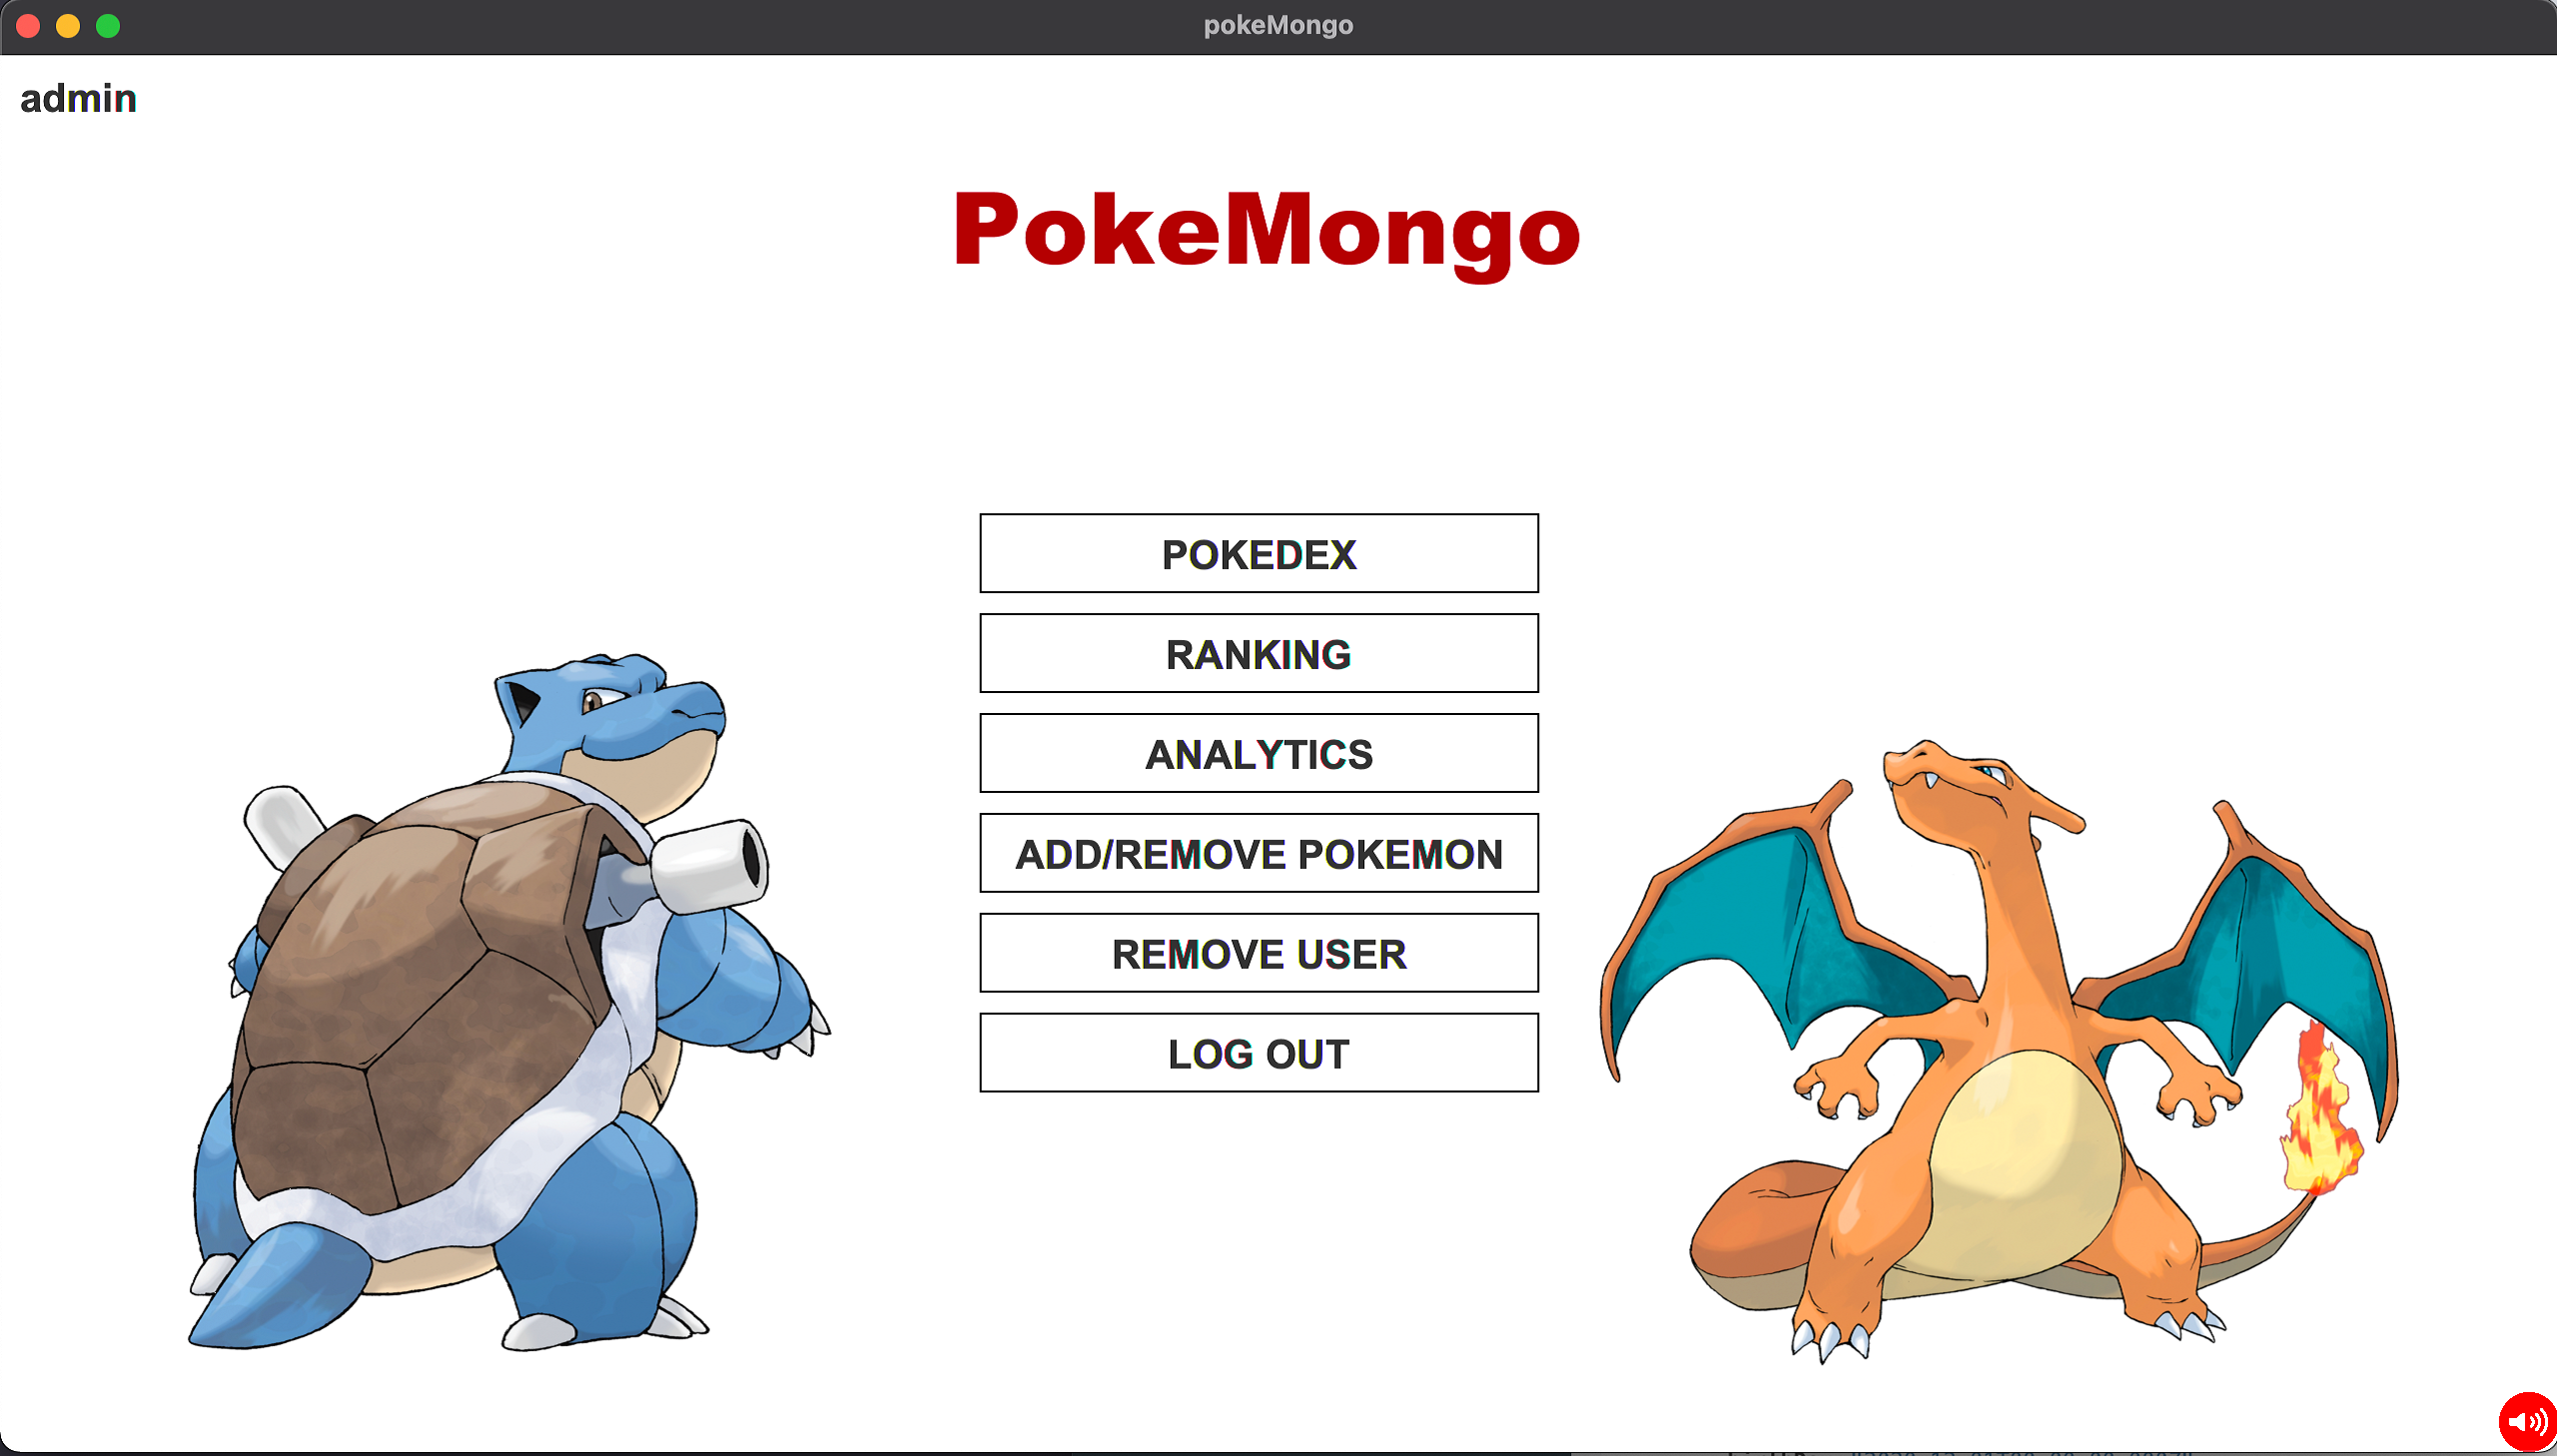
\includegraphics[width=\textwidth]{img/userManual/admin_homepage.png}
	\caption{Admin Homepage}
\end{figure}
Notice that the \textbf{Pokedex} page and the \textbf{Ranking} page are the same of the Normal User, with some slightly differences. Furthermore, the number of daily pokeball is not present, due to the fact that the admin could not play the catch'em all game, as we will se it would be unfair.
\subsubsection{Differences with Normal User}
By opening the Team Information Popup the admin has the possibility to delete some posts or replies as shown in the following figure, in which are presents some DELETE labels in each post or reply.
\begin{figure}[H]
	\centering
	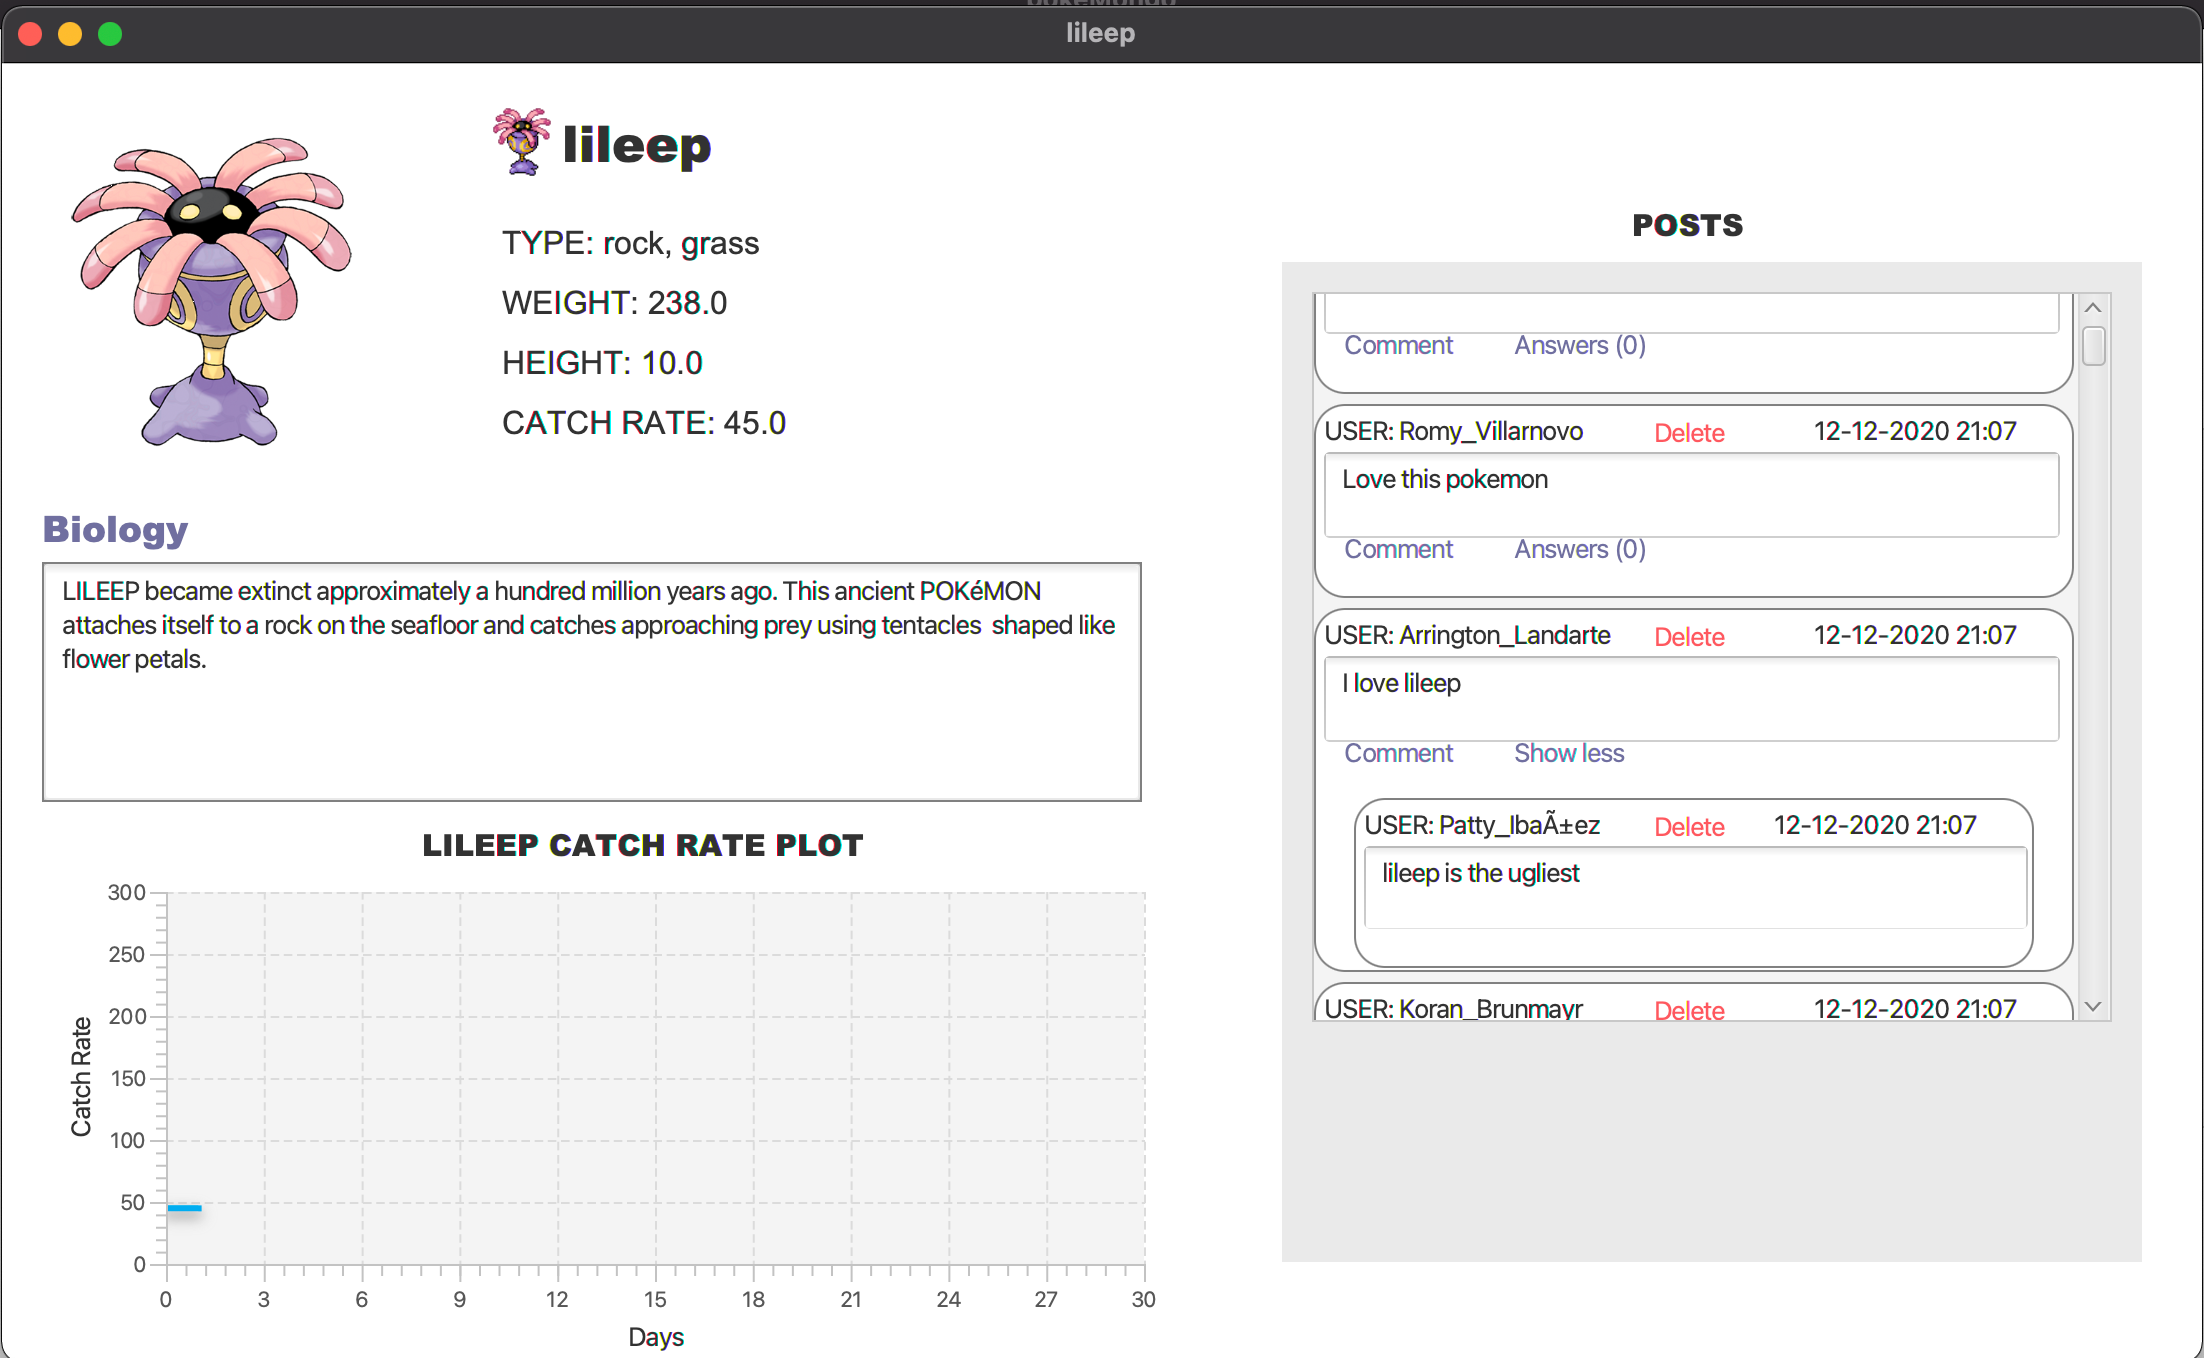
\includegraphics[width=\textwidth]{img/userManual/admin_pokemon_window.png}
	\caption{Admin Pokemon Popup}
\end{figure}
Moreover, in the ranking page, there is no ranking among friends because the admin can not have friends (FOLLOWING) or be friend (FOLLOWER) of someone.

\subsubsection{Analytics}
In the following page the \textbf{Admin} can have some insights about the usage statistics of the application. In fact, in the top-left plot there is plotted the number of total User in the last 30 days. On the bottom-left are plotted the number of daily logins in the last 30 days.
On the right there is a similar plot, which can be filtered by Country through the apposite combobox.
\begin{figure}[H]
	\centering
	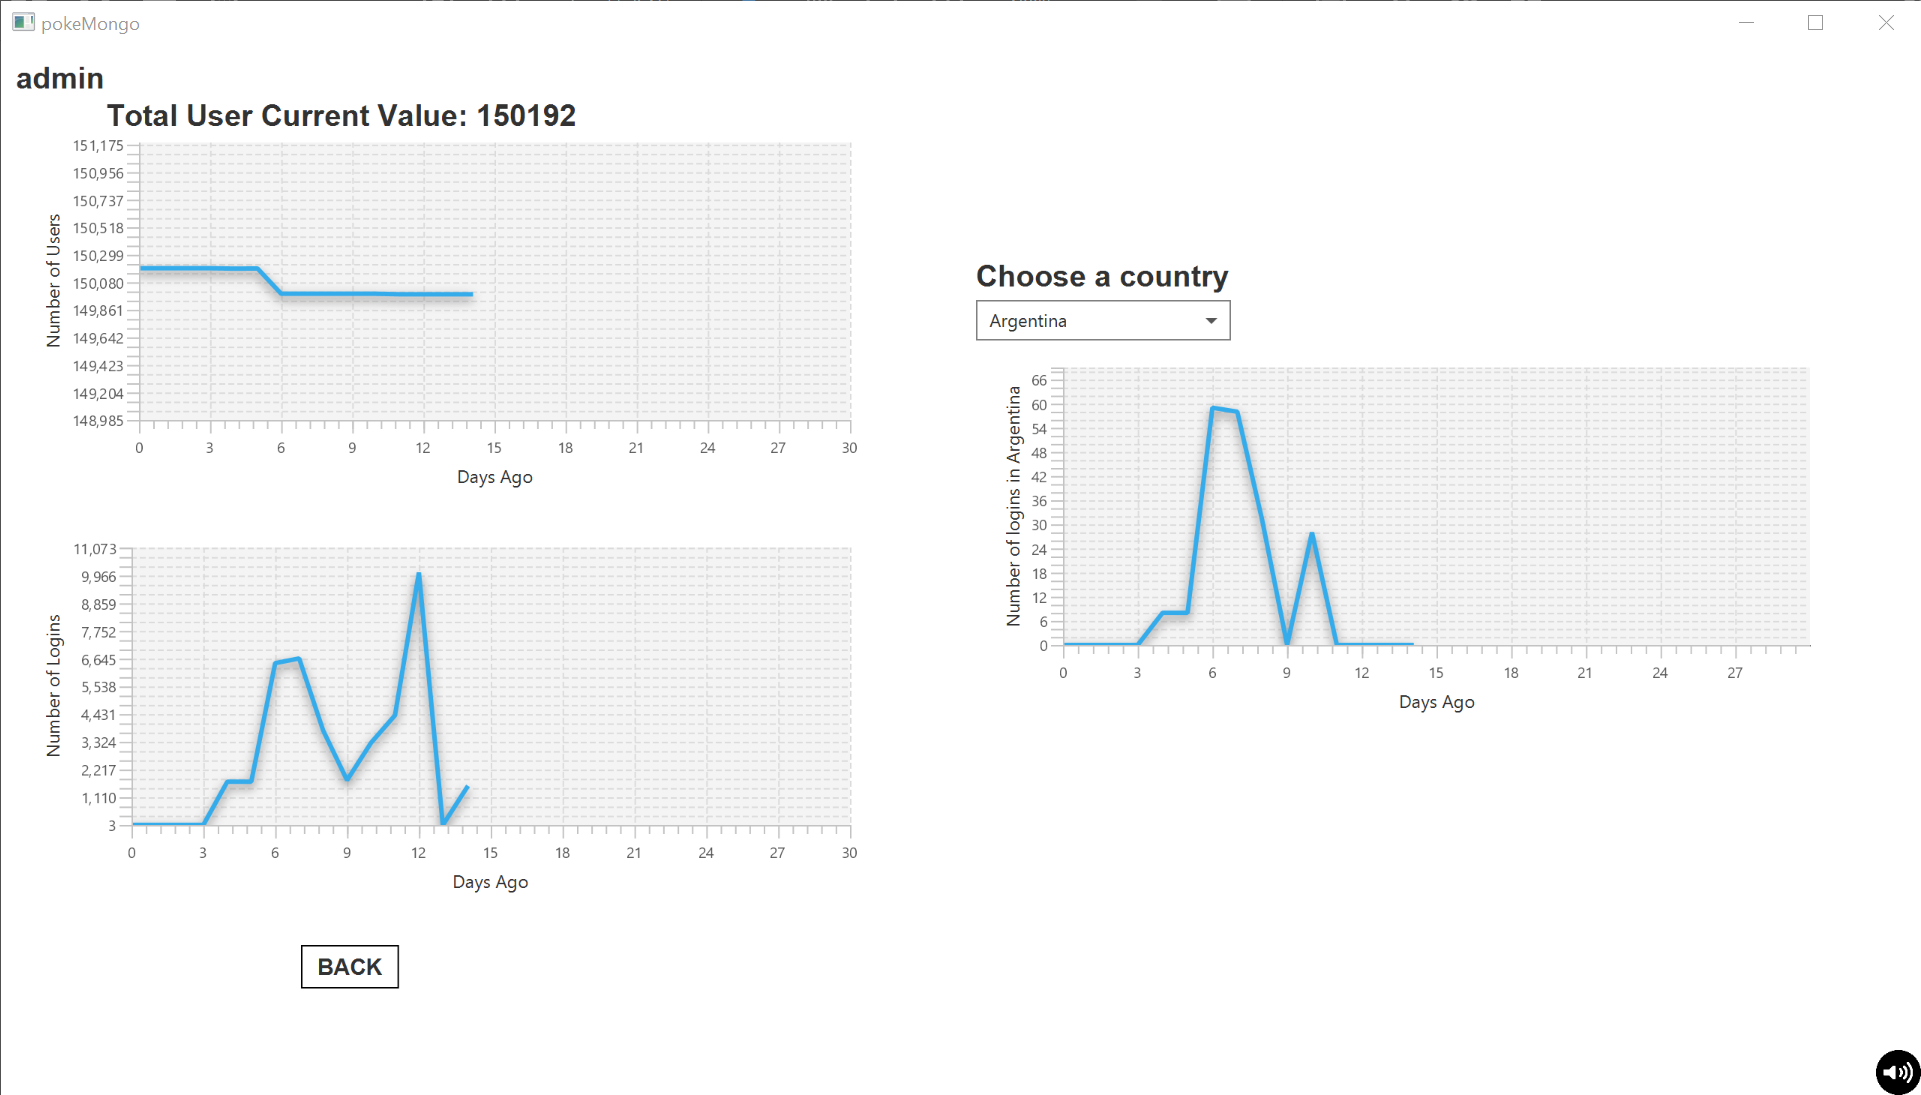
\includegraphics[width=\textwidth]{img/userManual/usage_statistics.png}
	\caption{Analytics Page}
\end{figure}

\subsubsection{Add/Remove Pokemon}
In this page, by clicking on one of the radio buttons on the top, is possible to delete or add a Pokemon in the system in order to update the application if there are some new \textbf{Pokemons} released by GameFreak or just some user-made ones. 
In order to add a pokemon, after selecting the radio button ADD POKEMON, the Admin must compile every field of the form, by adding even the urls of the images that will be shown. Then, he must click the ADD button and a green popup will be shown if the procedures have been made correctly. 
\begin{figure}[H]
	\centering
	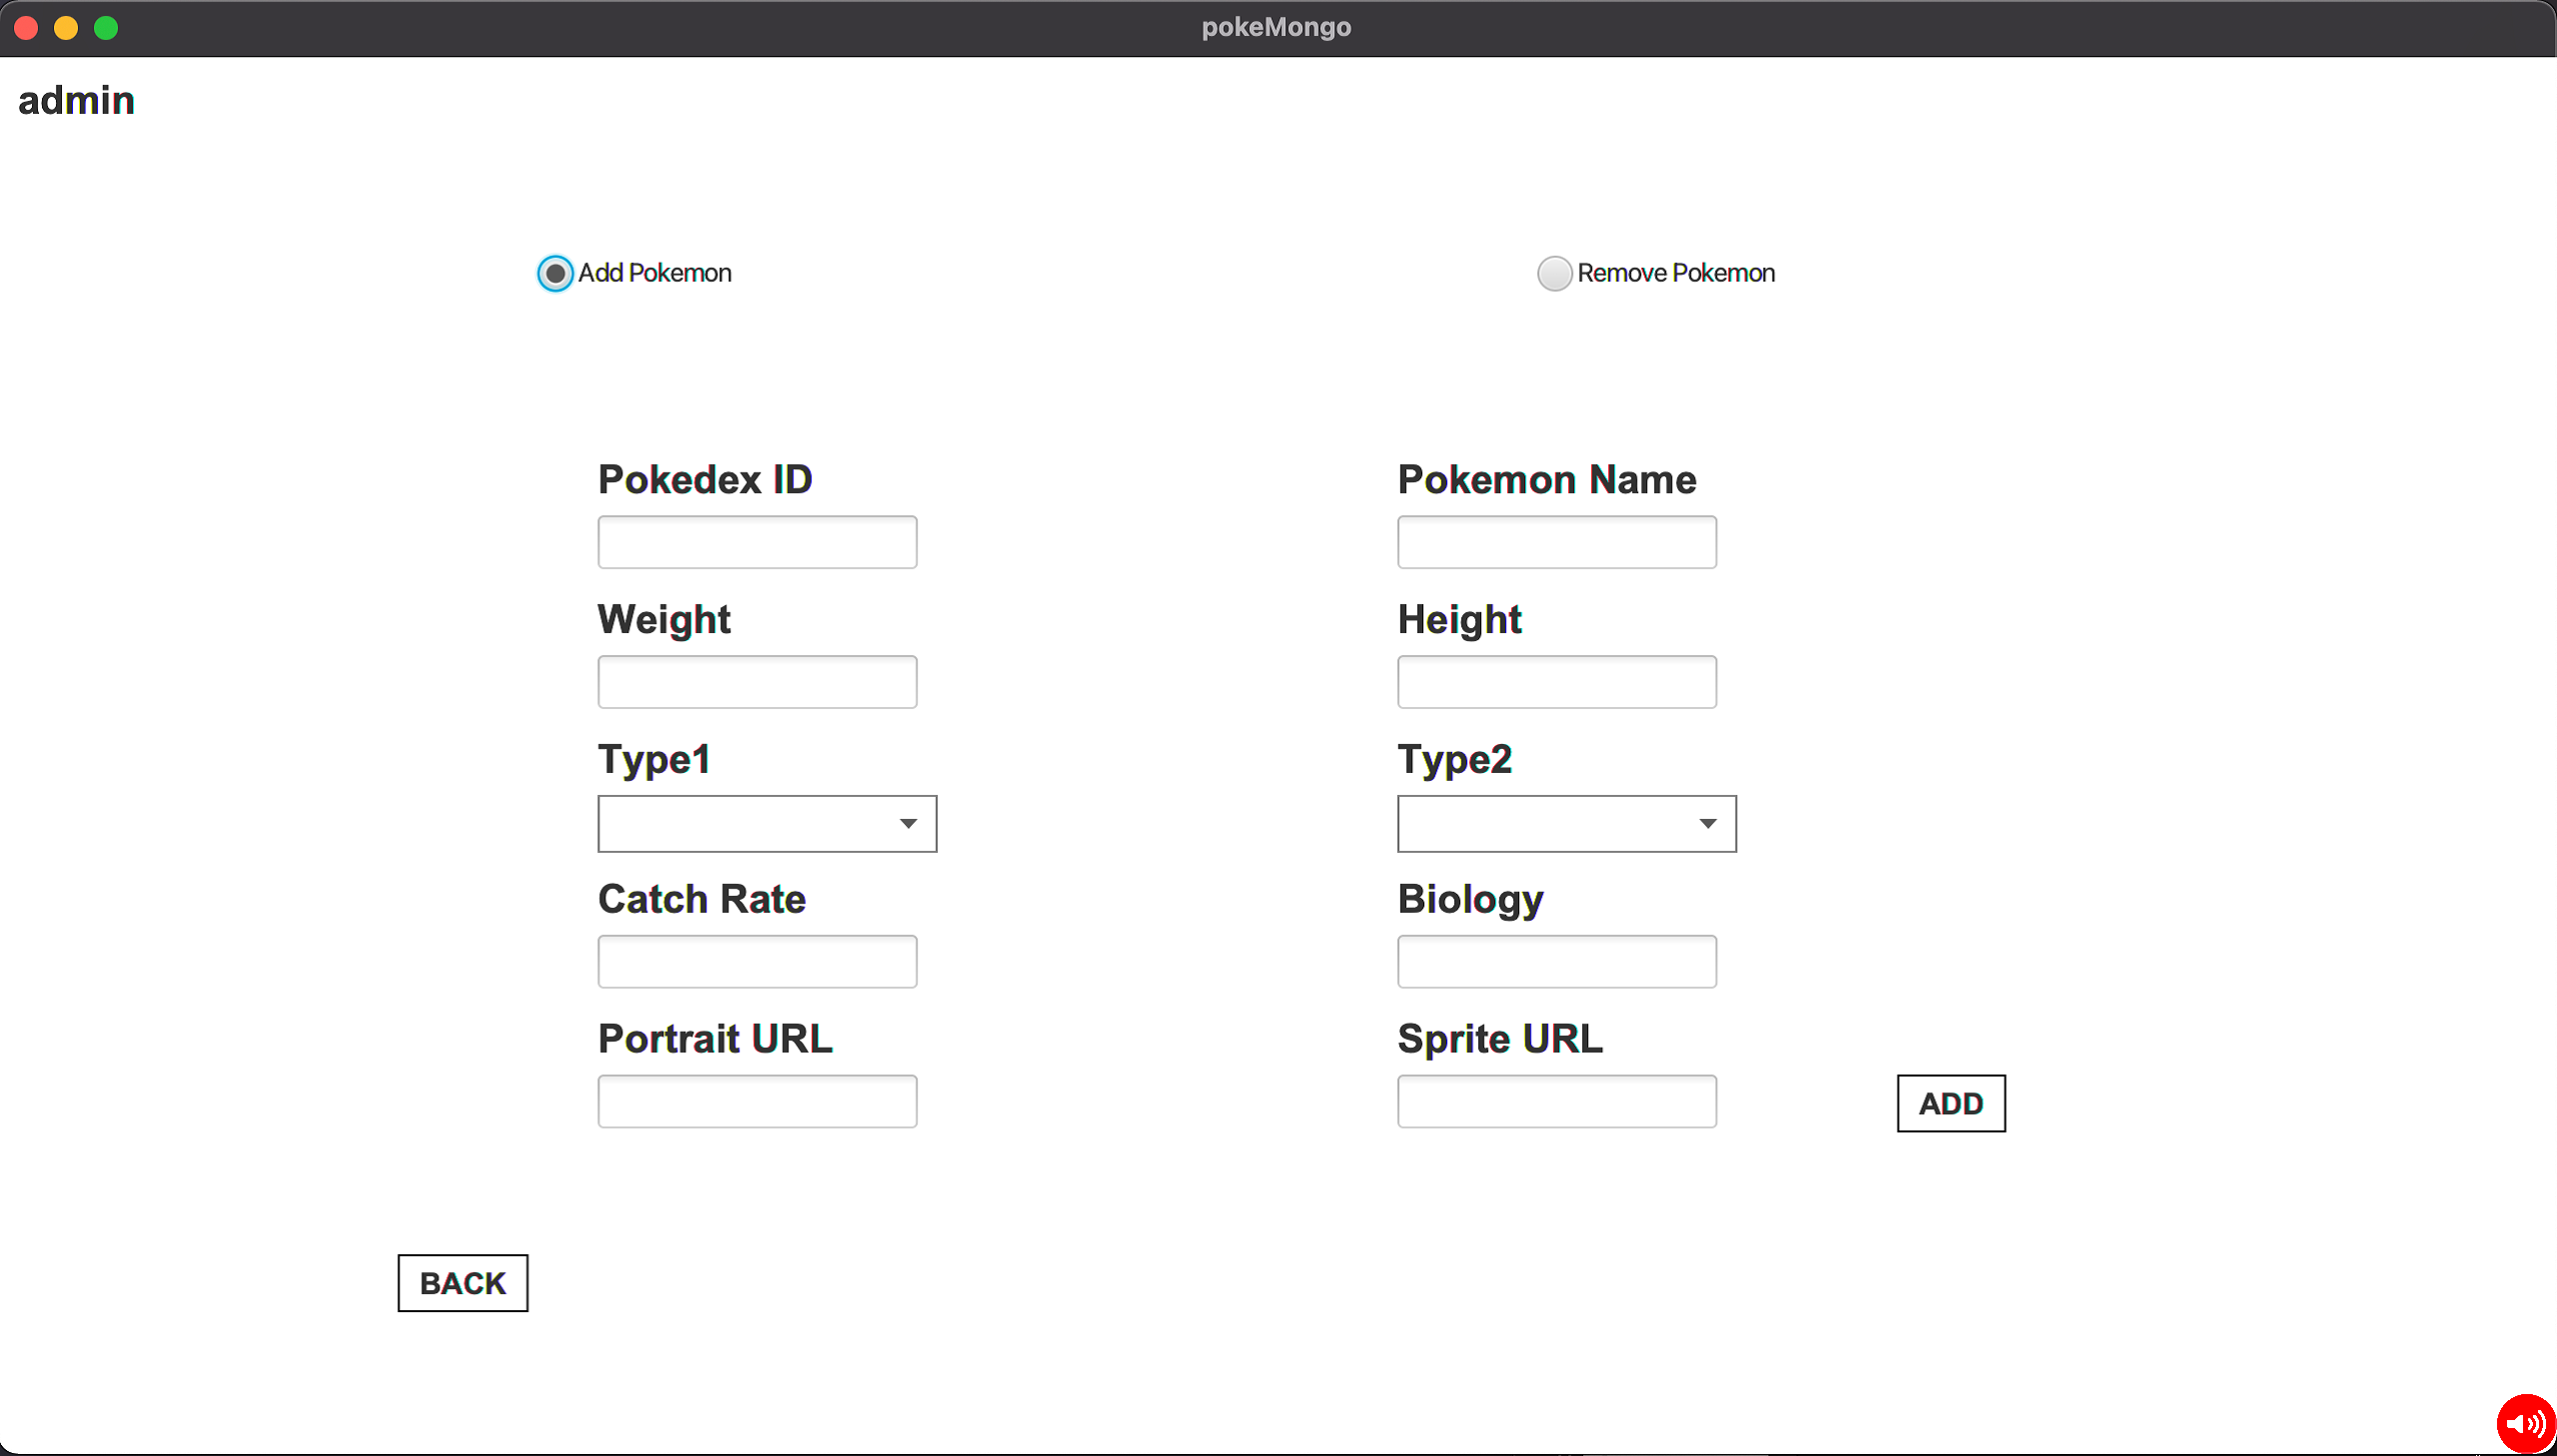
\includegraphics[width=\textwidth]{img/userManual/add_pokemon.png}
	\caption{Add Pokemon Page}
\end{figure}
For removing a pokemon is enough to write down the name of the pokemon and click the REMOVE button, a green popup will be showed in order to confirm the deletion.
\begin{figure}[H]
	\centering
	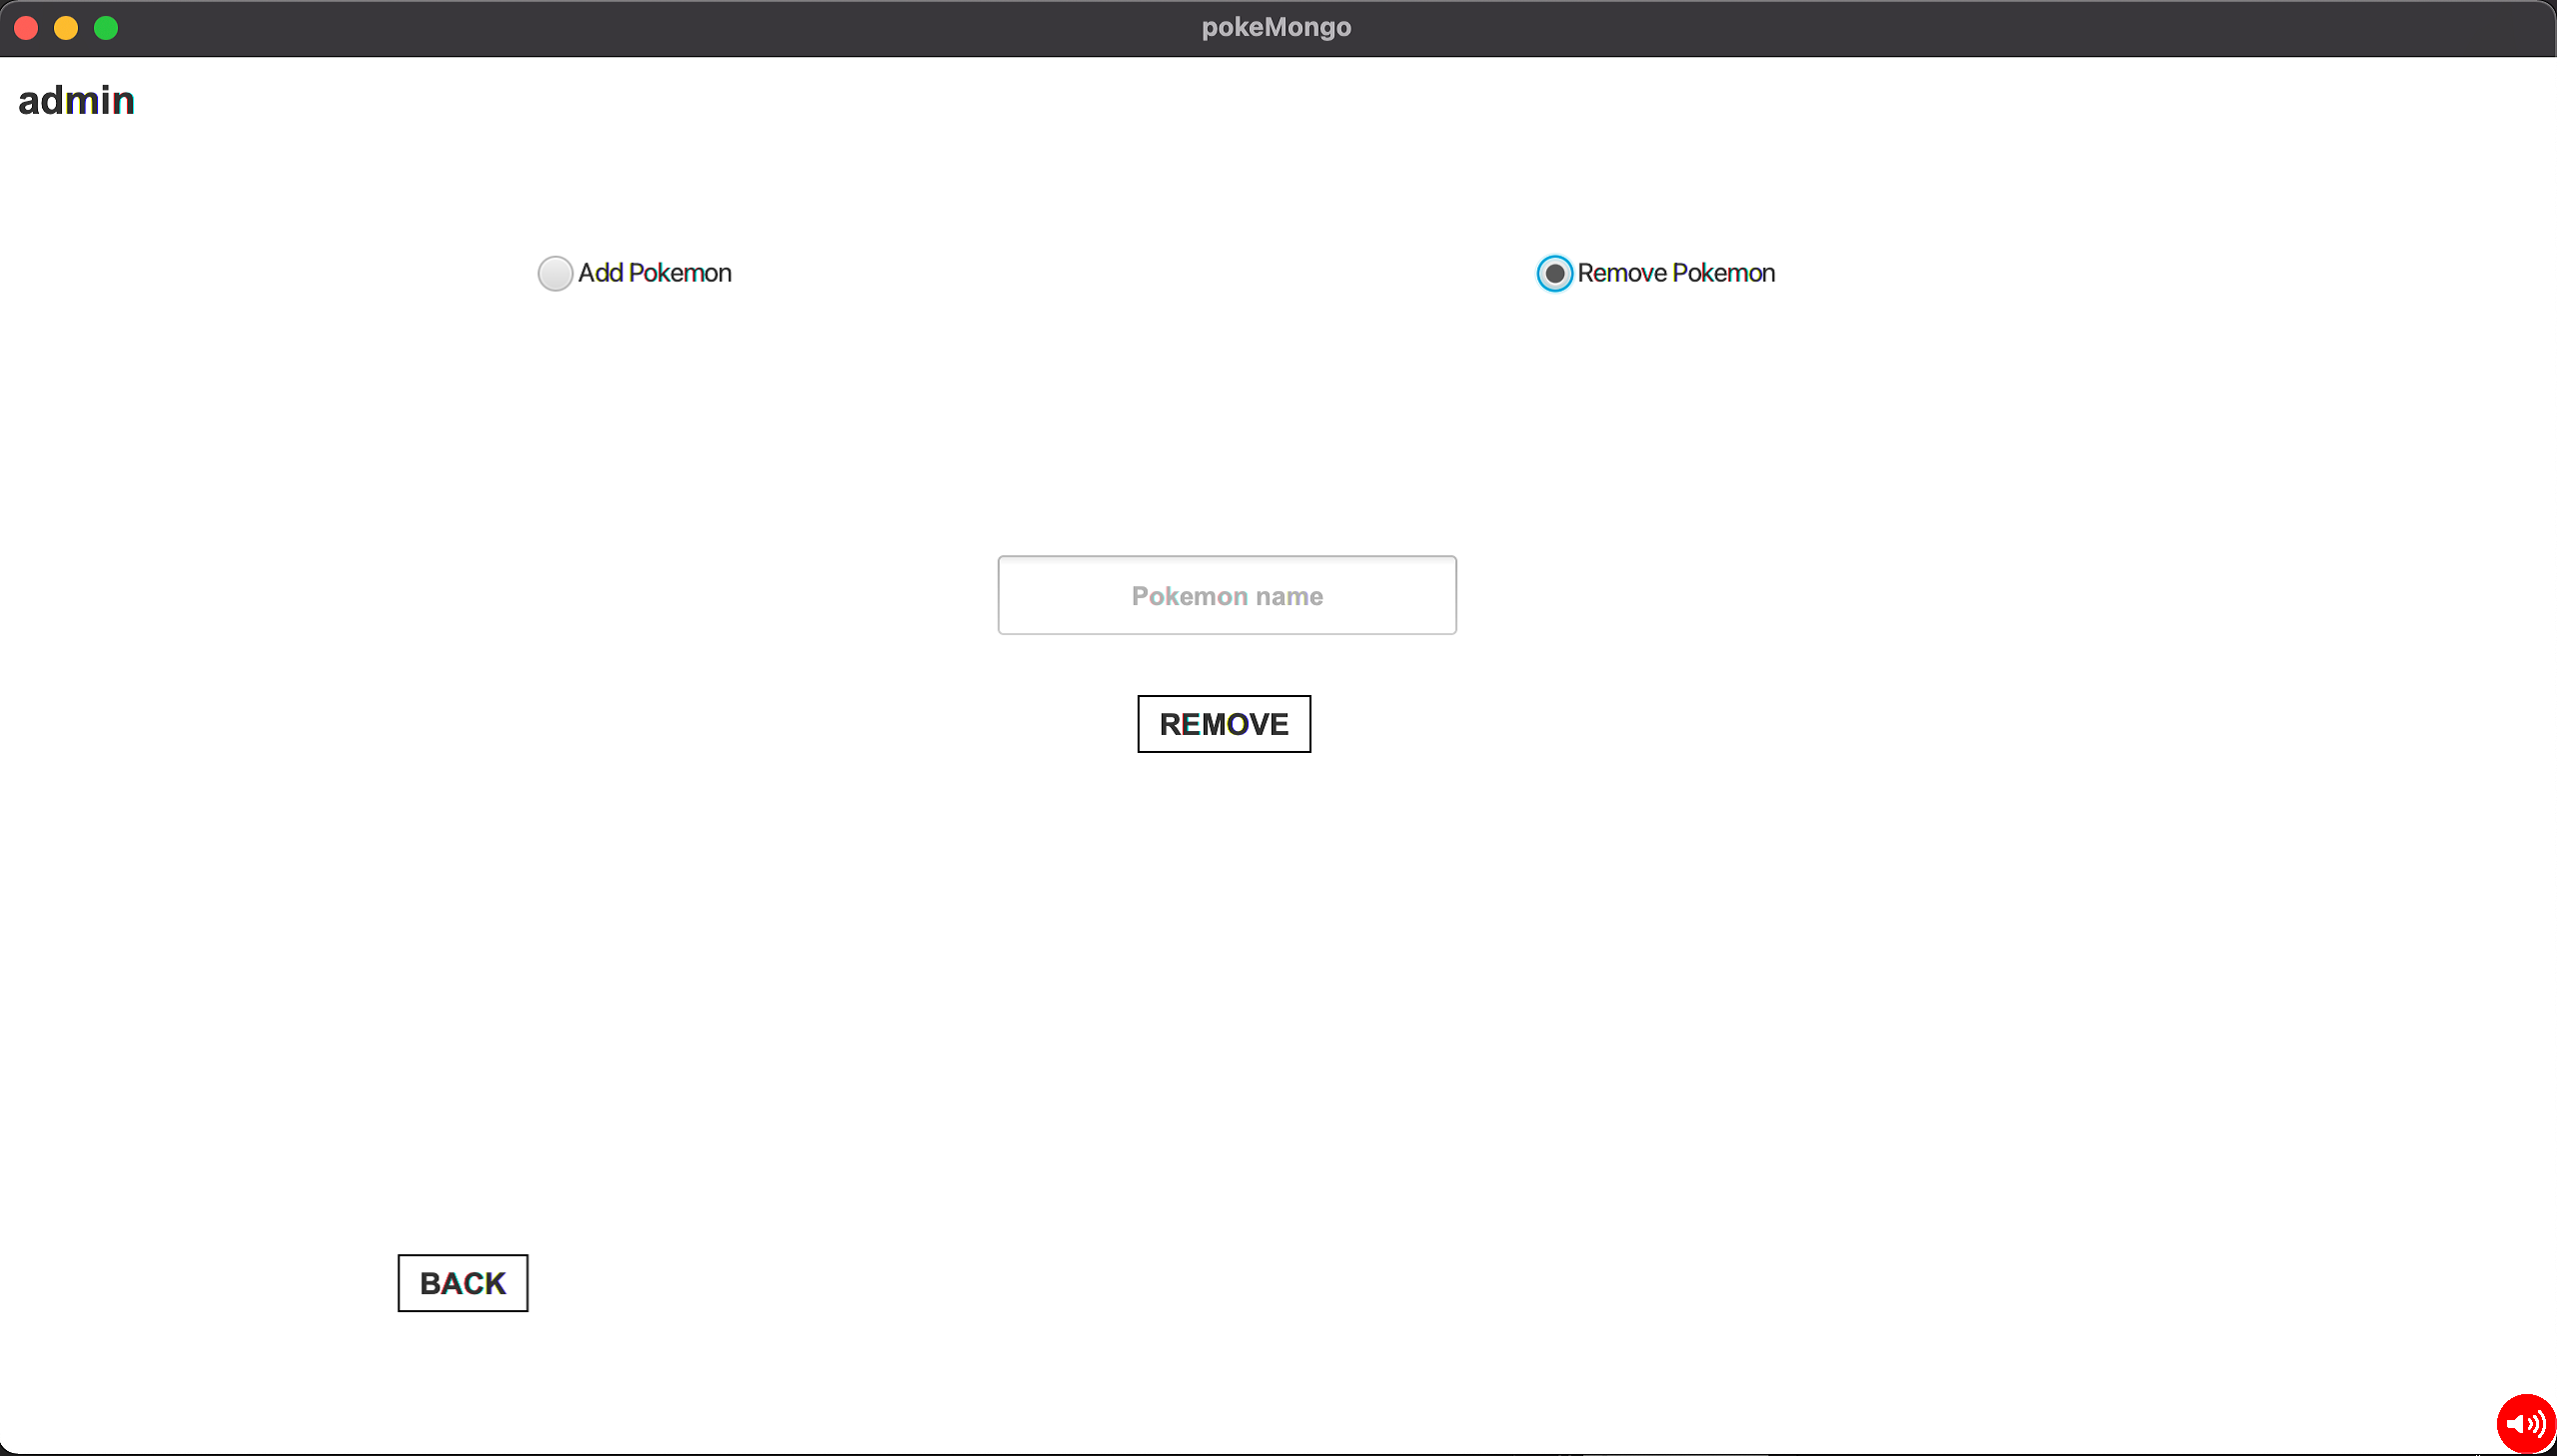
\includegraphics[width=\textwidth]{img/userManual/remove_pokemon.png}
	\caption{Remove Pokemon Page}
\end{figure}
\subsubsection{Remove Users}
An Admin can decide to ban a mischievous \textbf{User}. In order to do so, there is the \textbf{Delete User Page} in which, by just typing the username of that particular User and pressing the REMOVE button, the \textbf{User} will be removed from the system. If a green popup will be displayed, it will mean that the \textbf{User} deletion operation has been completed successfully. 
\begin{figure}[H]
	\centering
	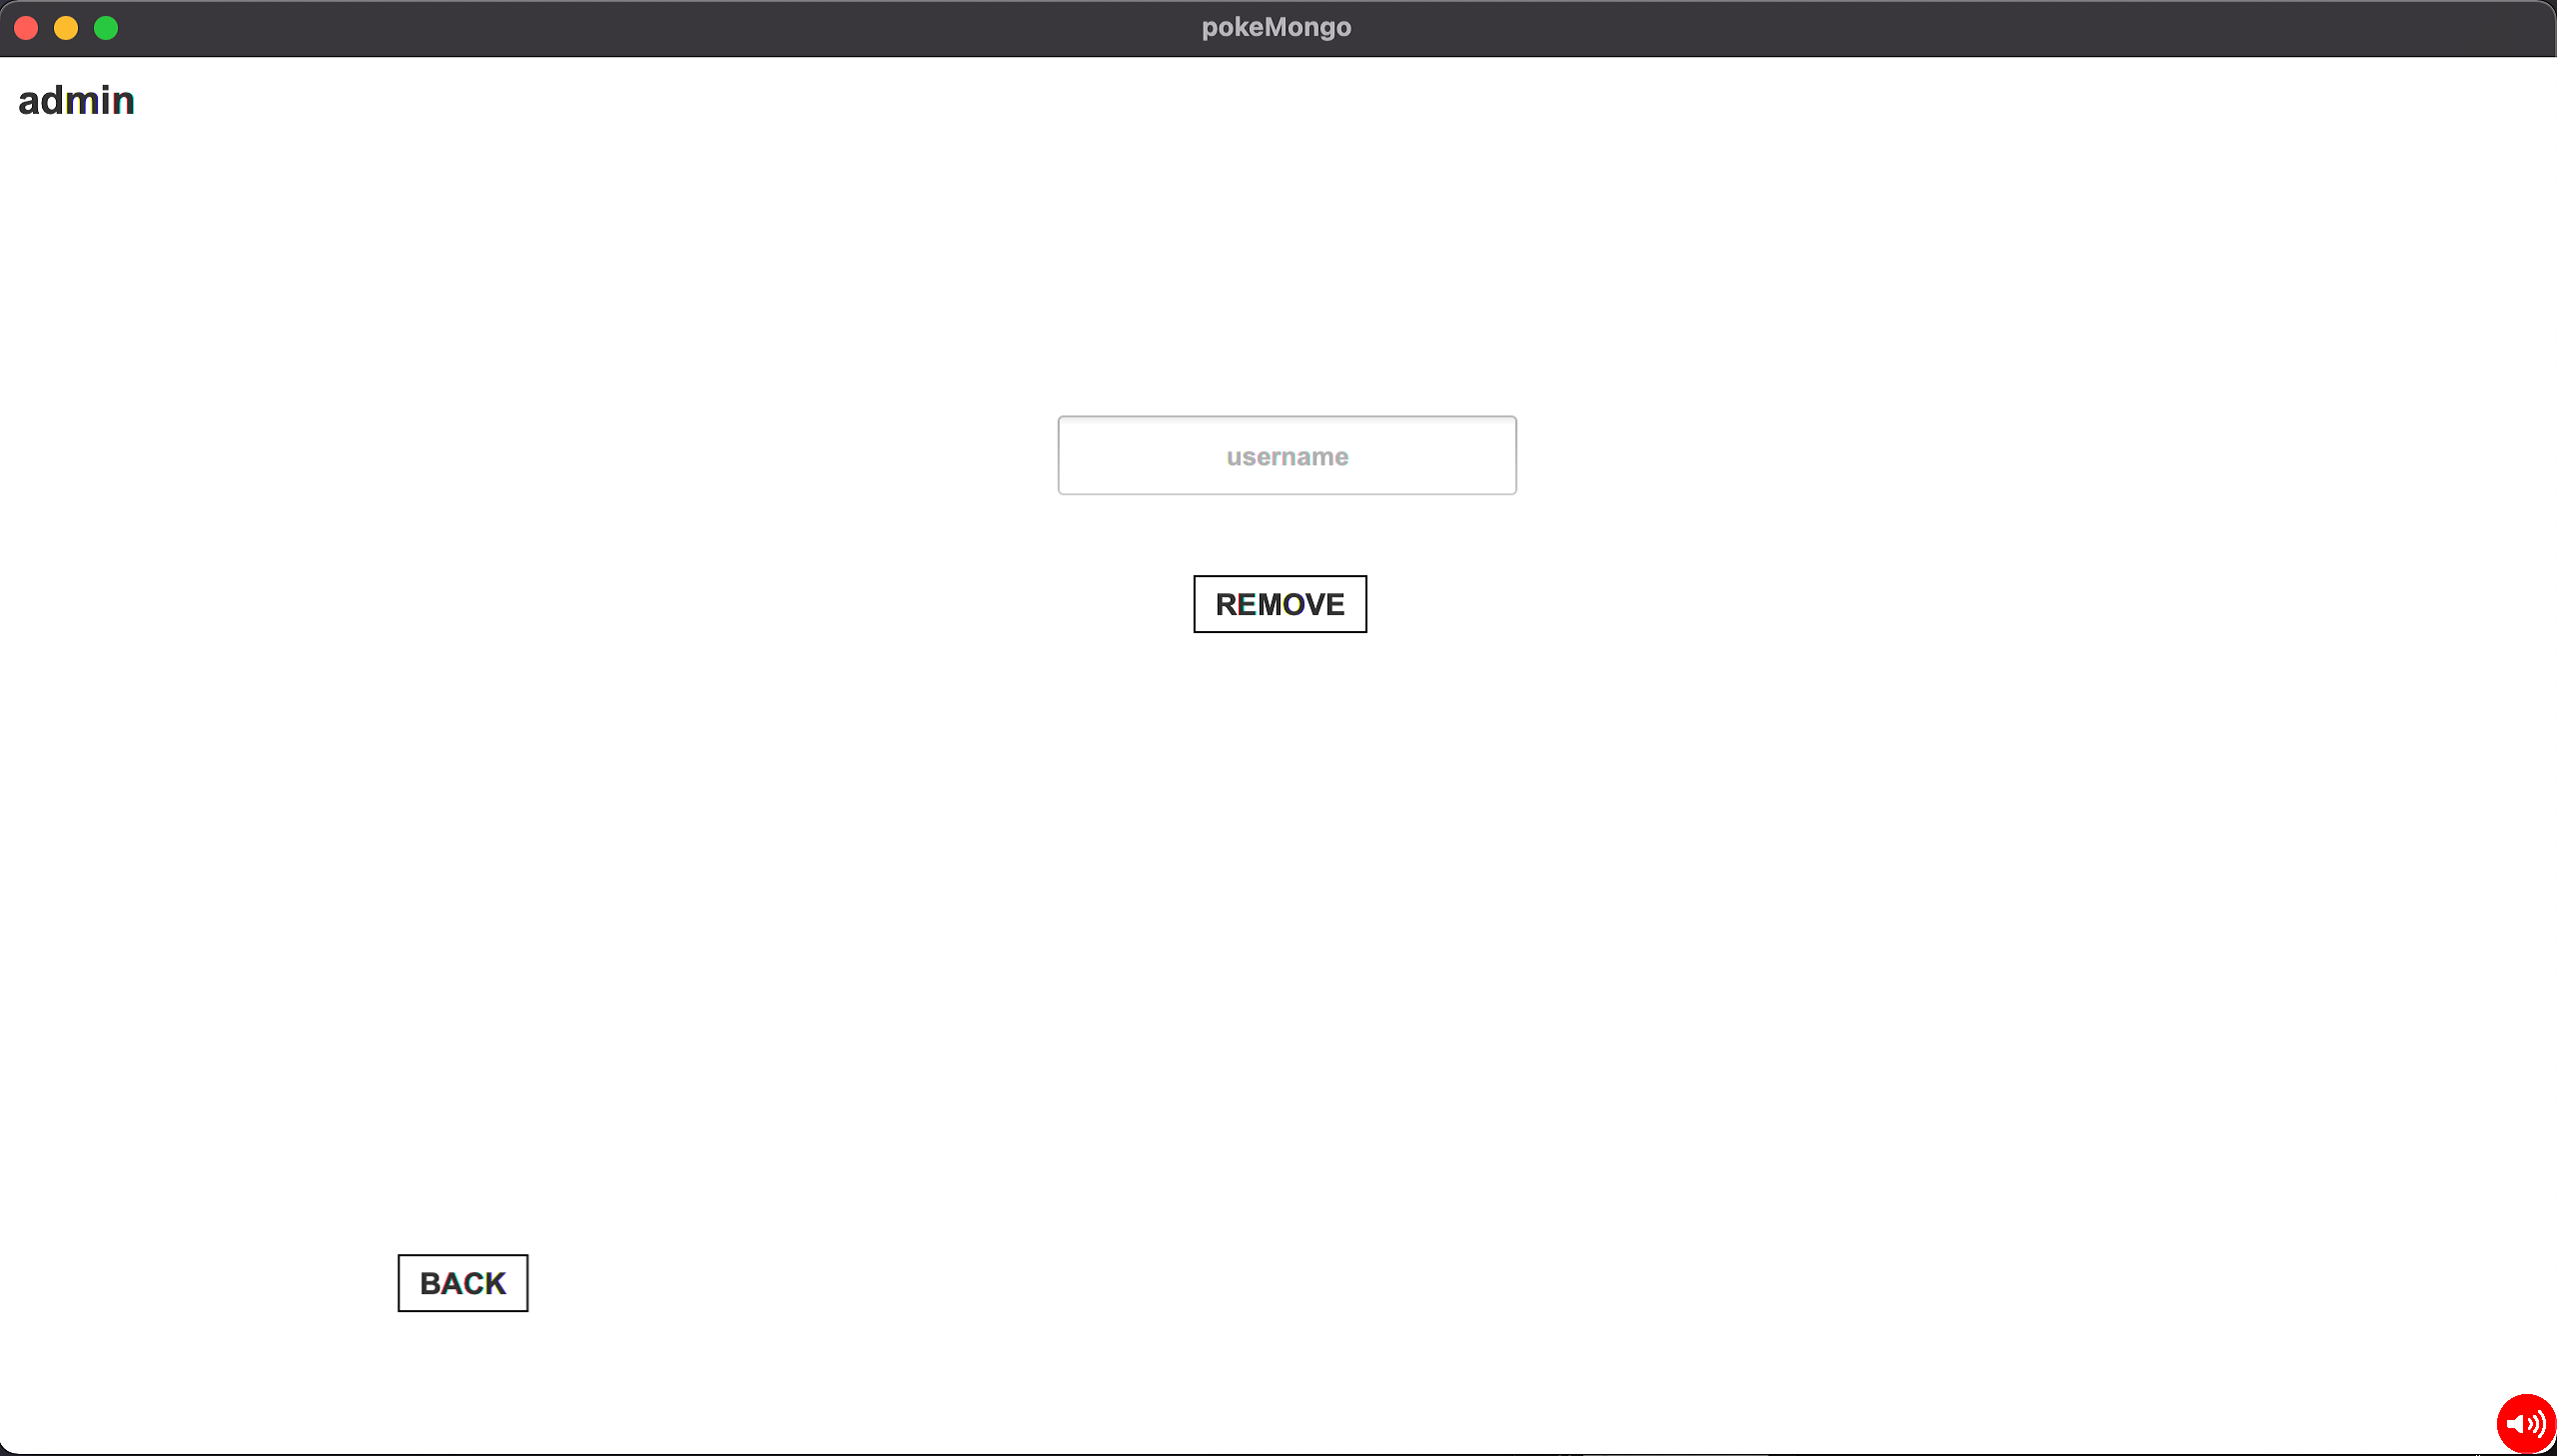
\includegraphics[width=\textwidth]{img/userManual/delete_user.png}
	\caption{Delete User Page}
\end{figure}